\documentclass[dvipsnames]{article} \usepackage[accepted]{icml2022}
\usepackage{tikz}
\usetikzlibrary{bayesnet}
\usepackage{xspace}
\usepackage{listings}
\usepackage{pifont}
\usepackage{paralist}
\usepackage{soul}
\newcommand{\cmark}{\ding{51}}\newcommand{\xmark}{\ding{55}}\usepackage{wrapfig}
\definecolor{lightgray}{gray}{0.9}

\usepackage[frozencache,cachedir=.]{minted}
\usepackage{listings}
\usepackage[compatibility=false]{caption}
\usepackage{microtype}
\usepackage{booktabs}
\usepackage[normalem]{ulem}
\usepackage{paralist}
\usepackage{mathtools}
\usepackage{xspace}
\usepackage{tikz}
\usepackage{amsmath}
\usepackage[colorlinks=true, allcolors=blue]{hyperref}
\usetikzlibrary{shapes,arrows}
\usetikzlibrary{positioning}
\usetikzlibrary{arrows.meta}
\usepackage{pgfplots}
\usepackage{cleveref}
\usepackage{subcaption}
\usepackage{booktabs}
\usepackage{tcolorbox}
\usepackage{amsmath,amsfonts,bm}
\newcommand{\figleft}{{\em (Left)}}
\newcommand{\figcenter}{{\em (Center)}}
\newcommand{\figright}{{\em (Right)}}
\newcommand{\figtop}{{\em (Top)}}
\newcommand{\figbottom}{{\em (Bottom)}}
\newcommand{\captiona}{{\em (a)}}
\newcommand{\captionb}{{\em (b)}}
\newcommand{\captionc}{{\em (c)}}
\newcommand{\captiond}{{\em (d)}}
\newcommand{\newterm}[1]{{\bf #1}}
\def\figref#1{figure~\ref{#1}}
\def\Figref#1{Figure~\ref{#1}}
\def\twofigref#1#2{figures \ref{#1} and \ref{#2}}
\def\quadfigref#1#2#3#4{figures \ref{#1}, \ref{#2}, \ref{#3} and \ref{#4}}
\def\secref#1{section~\ref{#1}}
\def\Secref#1{Section~\ref{#1}}
\def\twosecrefs#1#2{sections \ref{#1} and \ref{#2}}
\def\secrefs#1#2#3{sections \ref{#1}, \ref{#2} and \ref{#3}}
\def\eqref#1{equation~\ref{#1}}
\def\Eqref#1{Equation~\ref{#1}}
\def\plaineqref#1{\ref{#1}}
\def\chapref#1{chapter~\ref{#1}}
\def\Chapref#1{Chapter~\ref{#1}}
\def\rangechapref#1#2{chapters\ref{#1}--\ref{#2}}
\def\algref#1{algorithm~\ref{#1}}
\def\Algref#1{Algorithm~\ref{#1}}
\def\twoalgref#1#2{algorithms \ref{#1} and \ref{#2}}
\def\Twoalgref#1#2{Algorithms \ref{#1} and \ref{#2}}
\def\partref#1{part~\ref{#1}}
\def\Partref#1{Part~\ref{#1}}
\def\twopartref#1#2{parts \ref{#1} and \ref{#2}}

\def\ceil#1{\lceil #1 \rceil}
\def\floor#1{\lfloor #1 \rfloor}
\def\1{\bm{1}}
\newcommand{\train}{\mathcal{D}}
\newcommand{\valid}{\mathcal{D_{\mathrm{valid}}}}
\newcommand{\test}{\mathcal{D_{\mathrm{test}}}}

\def\eps{{\epsilon}}


\def\reta{{\textnormal{}}}
\def\ra{{\textnormal{a}}}
\def\rb{{\textnormal{b}}}
\def\rc{{\textnormal{c}}}
\def\rd{{\textnormal{d}}}
\def\re{{\textnormal{e}}}
\def\rf{{\textnormal{f}}}
\def\rg{{\textnormal{g}}}
\def\rh{{\textnormal{h}}}
\def\ri{{\textnormal{i}}}
\def\rj{{\textnormal{j}}}
\def\rk{{\textnormal{k}}}
\def\rl{{\textnormal{l}}}
\def\rn{{\textnormal{n}}}
\def\ro{{\textnormal{o}}}
\def\rp{{\textnormal{p}}}
\def\rq{{\textnormal{q}}}
\def\rr{{\textnormal{r}}}
\def\rs{{\textnormal{s}}}
\def\rt{{\textnormal{t}}}
\def\ru{{\textnormal{u}}}
\def\rv{{\textnormal{v}}}
\def\rw{{\textnormal{w}}}
\def\rx{{\textnormal{x}}}
\def\ry{{\textnormal{y}}}
\def\rz{{\textnormal{z}}}

\def\rvepsilon{{\mathbf{\epsilon}}}
\def\rvtheta{{\mathbf{\theta}}}
\def\rva{{\mathbf{a}}}
\def\rvb{{\mathbf{b}}}
\def\rvc{{\mathbf{c}}}
\def\rvd{{\mathbf{d}}}
\def\rve{{\mathbf{e}}}
\def\rvf{{\mathbf{f}}}
\def\rvg{{\mathbf{g}}}
\def\rvh{{\mathbf{h}}}
\def\rvu{{\mathbf{i}}}
\def\rvj{{\mathbf{j}}}
\def\rvk{{\mathbf{k}}}
\def\rvl{{\mathbf{l}}}
\def\rvm{{\mathbf{m}}}
\def\rvn{{\mathbf{n}}}
\def\rvo{{\mathbf{o}}}
\def\rvp{{\mathbf{p}}}
\def\rvq{{\mathbf{q}}}
\def\rvr{{\mathbf{r}}}
\def\rvs{{\mathbf{s}}}
\def\rvt{{\mathbf{t}}}
\def\rvu{{\mathbf{u}}}
\def\rvv{{\mathbf{v}}}
\def\rvw{{\mathbf{w}}}
\def\rvx{{\mathbf{x}}}
\def\rvy{{\mathbf{y}}}
\def\rvz{{\mathbf{z}}}

\def\erva{{\textnormal{a}}}
\def\ervb{{\textnormal{b}}}
\def\ervc{{\textnormal{c}}}
\def\ervd{{\textnormal{d}}}
\def\erve{{\textnormal{e}}}
\def\ervf{{\textnormal{f}}}
\def\ervg{{\textnormal{g}}}
\def\ervh{{\textnormal{h}}}
\def\ervi{{\textnormal{i}}}
\def\ervj{{\textnormal{j}}}
\def\ervk{{\textnormal{k}}}
\def\ervl{{\textnormal{l}}}
\def\ervm{{\textnormal{m}}}
\def\ervn{{\textnormal{n}}}
\def\ervo{{\textnormal{o}}}
\def\ervp{{\textnormal{p}}}
\def\ervq{{\textnormal{q}}}
\def\ervr{{\textnormal{r}}}
\def\ervs{{\textnormal{s}}}
\def\ervt{{\textnormal{t}}}
\def\ervu{{\textnormal{u}}}
\def\ervv{{\textnormal{v}}}
\def\ervw{{\textnormal{w}}}
\def\ervx{{\textnormal{x}}}
\def\ervy{{\textnormal{y}}}
\def\ervz{{\textnormal{z}}}

\def\rmA{{\mathbf{A}}}
\def\rmB{{\mathbf{B}}}
\def\rmC{{\mathbf{C}}}
\def\rmD{{\mathbf{D}}}
\def\rmE{{\mathbf{E}}}
\def\rmF{{\mathbf{F}}}
\def\rmG{{\mathbf{G}}}
\def\rmH{{\mathbf{H}}}
\def\rmI{{\mathbf{I}}}
\def\rmJ{{\mathbf{J}}}
\def\rmK{{\mathbf{K}}}
\def\rmL{{\mathbf{L}}}
\def\rmM{{\mathbf{M}}}
\def\rmN{{\mathbf{N}}}
\def\rmO{{\mathbf{O}}}
\def\rmP{{\mathbf{P}}}
\def\rmQ{{\mathbf{Q}}}
\def\rmR{{\mathbf{R}}}
\def\rmS{{\mathbf{S}}}
\def\rmT{{\mathbf{T}}}
\def\rmU{{\mathbf{U}}}
\def\rmV{{\mathbf{V}}}
\def\rmW{{\mathbf{W}}}
\def\rmX{{\mathbf{X}}}
\def\rmY{{\mathbf{Y}}}
\def\rmZ{{\mathbf{Z}}}

\def\ermA{{\textnormal{A}}}
\def\ermB{{\textnormal{B}}}
\def\ermC{{\textnormal{C}}}
\def\ermD{{\textnormal{D}}}
\def\ermE{{\textnormal{E}}}
\def\ermF{{\textnormal{F}}}
\def\ermG{{\textnormal{G}}}
\def\ermH{{\textnormal{H}}}
\def\ermI{{\textnormal{I}}}
\def\ermJ{{\textnormal{J}}}
\def\ermK{{\textnormal{K}}}
\def\ermL{{\textnormal{L}}}
\def\ermM{{\textnormal{M}}}
\def\ermN{{\textnormal{N}}}
\def\ermO{{\textnormal{O}}}
\def\ermP{{\textnormal{P}}}
\def\ermQ{{\textnormal{Q}}}
\def\ermR{{\textnormal{R}}}
\def\ermS{{\textnormal{S}}}
\def\ermT{{\textnormal{T}}}
\def\ermU{{\textnormal{U}}}
\def\ermV{{\textnormal{V}}}
\def\ermW{{\textnormal{W}}}
\def\ermX{{\textnormal{X}}}
\def\ermY{{\textnormal{Y}}}
\def\ermZ{{\textnormal{Z}}}

\def\vzero{{\bm{0}}}
\def\vone{{\bm{1}}}
\def\vmu{{\bm{\mu}}}
\def\vtheta{{\bm{\theta}}}
\def\va{{\bm{a}}}
\def\vb{{\bm{b}}}
\def\vc{{\bm{c}}}
\def\vd{{\bm{d}}}
\def\ve{{\bm{e}}}
\def\vf{{\bm{f}}}
\def\vg{{\bm{g}}}
\def\vh{{\bm{h}}}
\def\vi{{\bm{i}}}
\def\vj{{\bm{j}}}
\def\vk{{\bm{k}}}
\def\vl{{\bm{l}}}
\def\vm{{\bm{m}}}
\def\vn{{\bm{n}}}
\def\vo{{\bm{o}}}
\def\vp{{\bm{p}}}
\def\vq{{\bm{q}}}
\def\vr{{\bm{r}}}
\def\vs{{\bm{s}}}
\def\vt{{\bm{t}}}
\def\vu{{\bm{u}}}
\def\vv{{\bm{v}}}
\def\vw{{\bm{w}}}
\def\vx{{\bm{x}}}
\def\vy{{\bm{y}}}
\def\vz{{\bm{z}}}

\def\evalpha{{\alpha}}
\def\evbeta{{\beta}}
\def\evepsilon{{\epsilon}}
\def\evlambda{{\lambda}}
\def\evomega{{\omega}}
\def\evmu{{\mu}}
\def\evpsi{{\psi}}
\def\evsigma{{\sigma}}
\def\evtheta{{\theta}}
\def\eva{{a}}
\def\evb{{b}}
\def\evc{{c}}
\def\evd{{d}}
\def\eve{{e}}
\def\evf{{f}}
\def\evg{{g}}
\def\evh{{h}}
\def\evi{{i}}
\def\evj{{j}}
\def\evk{{k}}
\def\evl{{l}}
\def\evm{{m}}
\def\evn{{n}}
\def\evo{{o}}
\def\evp{{p}}
\def\evq{{q}}
\def\evr{{r}}
\def\evs{{s}}
\def\evt{{t}}
\def\evu{{u}}
\def\evv{{v}}
\def\evw{{w}}
\def\evx{{x}}
\def\evy{{y}}
\def\evz{{z}}

\def\mA{{\bm{A}}}
\def\mB{{\bm{B}}}
\def\mC{{\bm{C}}}
\def\mD{{\bm{D}}}
\def\mE{{\bm{E}}}
\def\mF{{\bm{F}}}
\def\mG{{\bm{G}}}
\def\mH{{\bm{H}}}
\def\mI{{\bm{I}}}
\def\mJ{{\bm{J}}}
\def\mK{{\bm{K}}}
\def\mL{{\bm{L}}}
\def\mM{{\bm{M}}}
\def\mN{{\bm{N}}}
\def\mO{{\bm{O}}}
\def\mP{{\bm{P}}}
\def\mQ{{\bm{Q}}}
\def\mR{{\bm{R}}}
\def\mS{{\bm{S}}}
\def\mT{{\bm{T}}}
\def\mU{{\bm{U}}}
\def\mV{{\bm{V}}}
\def\mW{{\bm{W}}}
\def\mX{{\bm{X}}}
\def\mY{{\bm{Y}}}
\def\mZ{{\bm{Z}}}
\def\mBeta{{\bm{\beta}}}
\def\mPhi{{\bm{\Phi}}}
\def\mLambda{{\bm{\Lambda}}}
\def\mSigma{{\bm{\Sigma}}}

\DeclareMathAlphabet{\mathsfit}{\encodingdefault}{\sfdefault}{m}{sl}
\SetMathAlphabet{\mathsfit}{bold}{\encodingdefault}{\sfdefault}{bx}{n}
\newcommand{\tens}[1]{\bm{\mathsfit{#1}}}
\def\tA{{\tens{A}}}
\def\tB{{\tens{B}}}
\def\tC{{\tens{C}}}
\def\tD{{\tens{D}}}
\def\tE{{\tens{E}}}
\def\tF{{\tens{F}}}
\def\tG{{\tens{G}}}
\def\tH{{\tens{H}}}
\def\tI{{\tens{I}}}
\def\tJ{{\tens{J}}}
\def\tK{{\tens{K}}}
\def\tL{{\tens{L}}}
\def\tM{{\tens{M}}}
\def\tN{{\tens{N}}}
\def\tO{{\tens{O}}}
\def\tP{{\tens{P}}}
\def\tQ{{\tens{Q}}}
\def\tR{{\tens{R}}}
\def\tS{{\tens{S}}}
\def\tT{{\tens{T}}}
\def\tU{{\tens{U}}}
\def\tV{{\tens{V}}}
\def\tW{{\tens{W}}}
\def\tX{{\tens{X}}}
\def\tY{{\tens{Y}}}
\def\tZ{{\tens{Z}}}


\def\gA{{\mathcal{A}}}
\def\gB{{\mathcal{B}}}
\def\gC{{\mathcal{C}}}
\def\gD{{\mathcal{D}}}
\def\gE{{\mathcal{E}}}
\def\gF{{\mathcal{F}}}
\def\gG{{\mathcal{G}}}
\def\gH{{\mathcal{H}}}
\def\gI{{\mathcal{I}}}
\def\gJ{{\mathcal{J}}}
\def\gK{{\mathcal{K}}}
\def\gL{{\mathcal{L}}}
\def\gM{{\mathcal{M}}}
\def\gN{{\mathcal{N}}}
\def\gO{{\mathcal{O}}}
\def\gP{{\mathcal{P}}}
\def\gQ{{\mathcal{Q}}}
\def\gR{{\mathcal{R}}}
\def\gS{{\mathcal{S}}}
\def\gT{{\mathcal{T}}}
\def\gU{{\mathcal{U}}}
\def\gV{{\mathcal{V}}}
\def\gW{{\mathcal{W}}}
\def\gX{{\mathcal{X}}}
\def\gY{{\mathcal{Y}}}
\def\gZ{{\mathcal{Z}}}

\def\sA{{\mathbb{A}}}
\def\sB{{\mathbb{B}}}
\def\sC{{\mathbb{C}}}
\def\sD{{\mathbb{D}}}
\def\sF{{\mathbb{F}}}
\def\sG{{\mathbb{G}}}
\def\sH{{\mathbb{H}}}
\def\sI{{\mathbb{I}}}
\def\sJ{{\mathbb{J}}}
\def\sK{{\mathbb{K}}}
\def\sL{{\mathbb{L}}}
\def\sM{{\mathbb{M}}}
\def\sN{{\mathbb{N}}}
\def\sO{{\mathbb{O}}}
\def\sP{{\mathbb{P}}}
\def\sQ{{\mathbb{Q}}}
\def\sR{{\mathbb{R}}}
\def\sS{{\mathbb{S}}}
\def\sT{{\mathbb{T}}}
\def\sU{{\mathbb{U}}}
\def\sV{{\mathbb{V}}}
\def\sW{{\mathbb{W}}}
\def\sX{{\mathbb{X}}}
\def\sY{{\mathbb{Y}}}
\def\sZ{{\mathbb{Z}}}

\def\emLambda{{\Lambda}}
\def\emA{{A}}
\def\emB{{B}}
\def\emC{{C}}
\def\emD{{D}}
\def\emE{{E}}
\def\emF{{F}}
\def\emG{{G}}
\def\emH{{H}}
\def\emI{{I}}
\def\emJ{{J}}
\def\emK{{K}}
\def\emL{{L}}
\def\emM{{M}}
\def\emN{{N}}
\def\emO{{O}}
\def\emP{{P}}
\def\emQ{{Q}}
\def\emR{{R}}
\def\emS{{S}}
\def\emT{{T}}
\def\emU{{U}}
\def\emV{{V}}
\def\emW{{W}}
\def\emX{{X}}
\def\emY{{Y}}
\def\emZ{{Z}}
\def\emSigma{{\Sigma}}

\newcommand{\etens}[1]{\mathsfit{#1}}
\def\etLambda{{\etens{\Lambda}}}
\def\etA{{\etens{A}}}
\def\etB{{\etens{B}}}
\def\etC{{\etens{C}}}
\def\etD{{\etens{D}}}
\def\etE{{\etens{E}}}
\def\etF{{\etens{F}}}
\def\etG{{\etens{G}}}
\def\etH{{\etens{H}}}
\def\etI{{\etens{I}}}
\def\etJ{{\etens{J}}}
\def\etK{{\etens{K}}}
\def\etL{{\etens{L}}}
\def\etM{{\etens{M}}}
\def\etN{{\etens{N}}}
\def\etO{{\etens{O}}}
\def\etP{{\etens{P}}}
\def\etQ{{\etens{Q}}}
\def\etR{{\etens{R}}}
\def\etS{{\etens{S}}}
\def\etT{{\etens{T}}}
\def\etU{{\etens{U}}}
\def\etV{{\etens{V}}}
\def\etW{{\etens{W}}}
\def\etX{{\etens{X}}}
\def\etY{{\etens{Y}}}
\def\etZ{{\etens{Z}}}

\newcommand{\pdata}{p_{\rm{data}}}
\newcommand{\ptrain}{\hat{p}_{\rm{data}}}
\newcommand{\Ptrain}{\hat{P}_{\rm{data}}}
\newcommand{\pmodel}{p_{\rm{model}}}
\newcommand{\Pmodel}{P_{\rm{model}}}
\newcommand{\ptildemodel}{\tilde{p}_{\rm{model}}}
\newcommand{\pencode}{p_{\rm{encoder}}}
\newcommand{\pdecode}{p_{\rm{decoder}}}
\newcommand{\precons}{p_{\rm{reconstruct}}}

\newcommand{\laplace}{\mathrm{Laplace}} 

\newcommand{\E}{\mathbb{E}}
\newcommand{\Ls}{\mathcal{L}}
\newcommand{\R}{\mathbb{R}}
\newcommand{\emp}{\tilde{p}}
\newcommand{\lr}{\alpha}
\newcommand{\reg}{\lambda}
\newcommand{\rect}{\mathrm{rectifier}}
\newcommand{\softmax}{\mathrm{softmax}}
\newcommand{\sigmoid}{\sigma}
\newcommand{\softplus}{\zeta}
\newcommand{\KL}{D_{\mathrm{KL}}}
\newcommand{\Var}{\mathrm{Var}}
\newcommand{\standarderror}{\mathrm{SE}}
\newcommand{\Cov}{\mathrm{Cov}}
\newcommand{\normlzero}{L^0}
\newcommand{\normlone}{L^1}
\newcommand{\normltwo}{L^2}
\newcommand{\normlp}{L^p}
\newcommand{\normmax}{L^\infty}

\newcommand{\parents}{Pa} 

\DeclareMathOperator*{\argmax}{arg\,max}
\DeclareMathOperator*{\argmin}{arg\,min}

\DeclareMathOperator{\sign}{sign}
\DeclareMathOperator{\Tr}{Tr}
\let\ab\allowbreak


\DeclareMathAlphabet\mathbfcal{OMS}{cmsy}{b}{n}
 \newcommand{\xx}[1]{\textsf{#1}\xspace}

\newcommand{\BS}[1]{
  \subsection*{\quad #1}
}

\let\labelindent\relax
\usepackage{enumitem} 
\newenvironment{enumpacked}{\begin{enumerate}[noitemsep,nolistsep,leftmargin=*]
}
{\end{enumerate}
}

\newenvironment{itempacked}{\begin{itemize}[noitemsep,nolistsep,leftmargin=*]
}
{\end{itemize}
}



\newcommand{\insight}[2]{
\begin{center}
\vspace{-1pt}
\framebox{
\parbox[c]{0.95\linewidth}{\it\sffamily #2}
}
\vspace{-3pt}
\end{center}
}

\newcommand{\tkooft}[1]{
\noindent
\framebox{
\begin{minipage}[c]{0.965\textwidth}
\it\sffamily#1
\end{minipage}
}
}

\newcommand{\lkooft}[1]{
\noindent
\framebox{
\parbox[c]{0.965\linewidth}{
\it\sffamily#1
}
}
}

\newcommand{\challenge}[1]{
\textsf{\it\sffamily#1}
}

\newcommand{\idea}[1]{
\insight{Idea}{#1}
}

\newcommand{\hemph}[1]{
\textbf{\sffamily#1}
}
\renewcommand{\bold}[1]{\textbf{\sffamily#1}}
\newcommand{\italic}[1]{\textit{\sffamily#1}}
\newcommand{\sans}[1]{{\sffamily#1}}

\newcommand{\ie}[0]{i.e.\xspace}

\newcommand{\hilite}[2]{\marginnote{\textcolor{blue}{#1}}\textcolor{red}{#2}\xspace}

\newcommand{\approxhl}[1]{{\footnotesize\colorbox{grayish}{\textbf{#1}}}\xspace}
\newcommand{\tline}[0]{\vspace{2pt}\hrule}
\newcommand{\bline}[0]{\vspace{-5pt}\hrule\vspace{2.5pt}}
\newcommand{\sfbold}[1]{{\small\sffamily\bfseries #1}}
\definecolor{grayish}{rgb}{0.85,0.85,0.85}

\newcommand{\benchmark}[1]{{\small\textsf{#1}}\normalsize\xspace}
\newcommand{\wire}[1]{{\bf\small\texttt{#1}}\normalsize\xspace}


\newcommand{\niparagraph}[1]{\vspace{1pt}\noindent\textbf{#1}}
\newcommand{\bench}[1]{{\textsf{#1}}\xspace}
\newcommand{\benchs}[1]{\bench{#1}s\xspace}
\newcommand{\code}[1]{\textsf{#1}}
\newcommand{\codes}[1]{\code{#1}s\xspace}
\newcommand{\sref}[1]{Section~\ref{section:#1}\xspace}
\newcommand{\fref}[1]{Figure~\ref{fig:#1}\xspace}
\newcommand{\tref}[1]{Table~\ref{table:#1}\xspace}
\newcommand{\eref}[1]{Equation~(\ref{eq:#1})\xspace}
\newcommand{\ldash}[0]{--}

\newcommand{\update}[2]{
\textcolor{blue}{\uwave{#2}\xsapce}
}
\newcommand{\highlight}[1]{\textcolor{BurntOrange}{#1}\xspace}

\newcommand{\fixme}[2]{\textcolor{BurntOrange}{#2}\xspace}
\newcommand{\takeout}[1]{\textcolor{Gray}{\uwave{#1}}\xspace}
\newcommand{\PrintTodo}{true}
\newcommand{\red}[1]{
\textcolor{red}{#1\xspace}
}

\newcommand{\new}[1]{{\color{blue}{\bf #1}}}
\newcommand*\circled[1]{\tikz[baseline=(char.base)]{
            \node[shape=circle,draw,fill=black,text=white,font=\sffamily\bfseries\small, inner sep=1.2pt] (char) {#1};}}

\newcommand{\finding}[1]{
\begin{center}
\noindent
\fbox{
  \parbox{0.98\linewidth}{
    \begin{center}
      \sf\bf\it #1
    \end{center}
  }
}
\end{center}
}

\newcommand{\cabstract}[1]{
\begin{center}
\begin{minipage}[c]{0.9\textwidth}
\singlespace\it\small
#1
\end{minipage}
\end{center}
}

\newcommand{\todo}[1]{\textcolor{red}{\textbf{TODO: #1}}}
\newcommand{\blue}[1]{\textcolor{blue}{#1}}
\newcommand{\TK}[1]{\textcolor{LimeGreen}{TK: #1}}
\newcommand{\GP}[1]{\textcolor{blue}{GP: #1}}

\newcommand\all[1]{\textcolor{blue}{ALL: #1}}

\newcommand{\newtext}[1]{\textcolor{brown}{#1}}
\newcommand{\ballnumber}[1]{\tikz[baseline=(myanchor.base)] \node[circle,fill=.,inner sep=1pt] (myanchor) {\color{-.}\bfseries\footnotesize #1};}




\newcommand{\aman}[1]{\textcolor{blue}{\textbf{\small[Aman: #1]}}}
\newcommand{\uri}[1]{\textcolor{OliveGreen}{\textbf{\small[Uri: #1]}}}
\newcommand{\luyu}[1]{\textcolor{Emerald}{\textbf{\small[Luyu: #1]}}}
\newcommand{\sz}[1]{\textcolor{Dandelion}{\textbf{\small[Shuyan: #1]}}}
\newcommand{\graham}[1]{\textcolor{red}{\textbf{\small[Graham: #1]}}}
\newcommand{\gn}[1]{\textcolor{red}{\textbf{\small[Graham: #1]}}}
\newcommand{\pengfei}[1]{\textcolor{RedOrange}{\textbf{\small[Pengfei: #1]}}}
\newcommand{\yiming}[1]{\textcolor{red}{\textbf{\small[Yiming: #1]}}}
\newcommand{\jamie}[1]{\textcolor{red}{\textbf{\small[Jamie: #1]}}}

\renewcommand{\aman}[1]{}
\renewcommand{\uri}[1]{}
\renewcommand{\luyu}[1]{}
\renewcommand{\sz}[1]{}
\renewcommand{\graham}[1]{}
\renewcommand{\gn}[1]{}
\renewcommand{\pengfei}[1]{}
\renewcommand{\yiming}[1]{}
\renewcommand{\jamie}[1]{}



 

\newcommand{\ours}{\textsc{PaL}\xspace}

\newcommand{\eg}{\textit{e.g.,}\xspace}


\newcommand{\model}{\xspace}
\newcommand{\pcond}[2]{p(#1 \mid #2)}
\newcommand{\prompt}{\xspace}
\newcommand{\concat}{\mathbin\Vert}

\newcommand{\interalia}[1]{\citep[\textit{inter alia}]{#1}}
\newcommand{\inlineCode}[1]{\texttt{{#1}}}
\newcommand{\hypho}[1]{\guillemotleft\guillemotright{}\xspace}
\newcommand{\cotp}{\textsc{CoT}\xspace}
\newcommand{\tomost}{\textsc{Least-to-Most}\xspace}
\newcommand{\direct}{\textsc{Direct}\xspace}
\newcommand{\llm}{LLM\xspace}
\newcommand{\llms}{LLMs\xspace}

\newcommand{\sports}{\textsc{Sports}\xspace}
\newcommand{\maths}{\textsc{Maths}\xspace}

\newcommand{\commonsense}{\textsc{Commonsense}\xspace}
\newcommand{\symbolic}{\textsc{Symbolic}\xspace}
\newcommand{\mathematical}{\textsc{Mathematical}\xspace}

\newcommand{\mathematicalbold}{\textsc{\textbf{Mathematical}}\xspace}
\newcommand{\commonsensebold}{\textsc{\textbf{Commonsense}}\xspace}

\newcommand{\datet}{\textsc{date}\xspace}
\newcommand{\gsm}{\textsc{gsm8k}\xspace}
\newcommand{\gsmhard}{\textsc{gsm-hard}\xspace}
\newcommand{\dropfb}{\textsc{drop}\xspace}
\newcommand{\dropnb}{\textsc{drop}\xspace}
\newcommand{\drop}{\textsc{drop-math}\xspace}
\newcommand{\multiarith}{\textsc{multiarith}\xspace}
\newcommand{\singleop}{\textsc{singleop}\xspace}
\newcommand{\singleeq}{\textsc{singleeq}\xspace}
\newcommand{\addsub}{\textsc{addsub}\xspace}
\newcommand{\asdiv}{\textsc{asdiv}\xspace}
\newcommand{\svamp}{\textsc{svamp}\xspace}
\newcommand{\mawps}{\textsc{mawps}\xspace}
\newcommand{\repeatcopy}{\textsc{Repeat Copy}\xspace}
\newcommand{\objectcounting}{\textsc{Object Counting}\xspace}

\newcommand{\csqa}{\textsc{csqa}\xspace}
\newcommand{\sorting}{\textsc{Sorting}\xspace}

 

\newcommand{\palm}{\textsc{P}a\textsc{LM}\xspace}
\newcommand{\smlpalm}{\textsc{P}a\textsc{LM}\textsc{-8b}\xspace}
\newcommand{\medpalm}{\textsc{P}a\textsc{LM}\textsc{-62b}\xspace}
\newcommand{\largepalm}{\textsc{P}a\textsc{LM}\textsc{-540b}\xspace}
\newcommand{\gptt}{\textsc{GPT-3}\xspace}
\newcommand{\codex}{\textsc{Codex}\xspace}

\newcommand{\sparam}{\textsc{8b}\xspace}
\newcommand{\mparam}{\textsc{62b}\xspace}
\newcommand{\lparam}{\textsc{540b}\xspace}

\newcommand{\spalm}{\smlpalm}
\newcommand{\mpalm}{\medpalm}
\newcommand{\lpalm}{\largepalm}

\newcommand{\running}{\red{\textsc{running}}}
\definecolor{codepurple}{rgb}{0.58,0,0.82}

\newcommand{\corr}[2]{\textbf{\textcolor{codepurple}{\st{#1} #2}}}

\newcommand{\Atwo}[3][A]{\begin{tikzpicture}
    \begin{scope}
      \node[inner sep=0pt,outer sep=0pt] (a) {\phantom{#1}};
      \clip (a.south west) rectangle ();
      \node[inner sep=0pt,outer sep=0pt,text=#2]  {#1};
    \end{scope}
    \clip (a.south east) rectangle ();
      \node[inner sep=0pt,outer sep=0pt,text=#3]  {#1};
  \end{tikzpicture}
}


\definecolor{cotcolor}{HTML}{56C1FF}
\definecolor{parcolortext}{HTML}{E01E5A}
\definecolor{parcolorback}{HTML}{E6E6E6}
\fboxsep=1pt \usepackage{float}
\usepackage{color}
\definecolor{deepblue}{rgb}{0,0,0.5}
\definecolor{deepred}{rgb}{0.6,0,0}
\definecolor{deepgreen}{rgb}{0,0.5,0}
\definecolor{darkgreen}{RGB}{43,163,39}
\definecolor{bluesquare}{rgb}{126,166,224}
\definecolor{LightGray}{gray}{0.9}
\definecolor{DarkGray}{gray}{0.1}

\renewcommand{\tt}[1]{\fontfamily{cmtt}\selectfont #1}


\lstdefinestyle{pythoncode}{
	language=Python,
	otherkeywords={self,join,append,split,write},   keywordstyle=\bfseries\color{deepblue},
	emph={__init__, digraph},          emphstyle=\color{deepred},    showstringspaces=false,
	breaklines=true,
	escapeinside=||,
	columns=fullflexible,
	basicstyle=\fontfamily{cmtt}\normalsize,
    belowskip=-\baselineskip,
    aboveskip=-0.7\baselineskip
}



\definecolor{codegreen}{rgb}{0,0.6,0}
\definecolor{codegray}{rgb}{0.5,0.5,0.5}
\definecolor{codepurple}{rgb}{0.58,0,0.82}
\definecolor{backcolour}{rgb}{0.95,0.95,0.92}



\newcommand{\classref}[1]{\textbf{\color{blue}{#1}}}
\newcommand{\funcname}[1]{\color{brown!50!black}{#1}}
\newcommand{\varref}[1]{\color{blue}{#1}}
\newcommand{\paren}[1]{\textbf{\color{magenta}{#1}}}
 

\PassOptionsToPackage{dvipsnames}{xcolor}
\definecolor{lightgray}{gray}{0.9}


  
  


\usepackage{minitoc}


\begin{document}



\twocolumn[
\icmltitle{PAL: Program-aided Language Models}
\icmltitlerunning{~ \hfill PAL: Program-aided Language Models \hfill \thepage}

\icmlsetsymbol{equal}{*}

\begin{icmlauthorlist}
\icmlauthor{Luyu Gao}{equal,lti}
\icmlauthor{Aman Madaan}{equal,lti}
\icmlauthor{Shuyan Zhou}{equal,lti}
\icmlauthor{Uri Alon}{lti}
\icmlauthor{Pengfei Liu}{lti,ic}
\icmlauthor{Yiming Yang}{lti}
\icmlauthor{Jamie Callan}{lti}
\icmlauthor{Graham Neubig}{lti,ic} \\
\begin{tabular}{c}
    \texttt{\{luyug,amadaan,shuyanzh,ualon,pliu3,yiming,callan,gneubig\}@cs.cmu.edu}
   \end{tabular} 
\end{icmlauthorlist}


\icmlaffiliation{lti}{Language Technologies Institute, Carnegie Mellon University, USA}
\icmlaffiliation{ic}{Inspired Cognition, USA}

\icmlcorrespondingauthor{Firstname1 Lastname1}{first1.last1@xxx.edu}
\icmlcorrespondingauthor{Firstname2 Lastname2}{first2.last2@www.uk}


\icmlkeywords{Machine Learning, ICML}
\vskip 0.3in
]
\printAffiliationsAndNotice{\icmlEqualContribution}

\begin{abstract}
Large language models (LLMs) have recently demonstrated an impressive ability to perform arithmetic and symbolic reasoning tasks, when provided with a few examples at test time (``few-shot prompting''). 
Much of this success can be attributed to prompting methods such as ``chain-of-thought'', which employ \llms for both \emph{understanding} the problem description by decomposing it into steps, as well as \emph{solving} each step of the problem.
While LLMs seem to be adept at this sort of step-by-step decomposition, LLMs often make logical and arithmetic mistakes in the solution part, even when the problem is decomposed correctly.
In this paper, we present Program-Aided Language models~(\ours): a novel approach that uses the LLM to read natural language problems and generate \emph{programs} as the intermediate reasoning steps, but offloads the \emph{solution} step to a runtime such as a Python interpreter.
With \ours, decomposing the natural language problem into runnable steps remains the only learning task for the \llm, while solving is delegated to the interpreter.
We demonstrate this synergy between a neural LLM and a symbolic interpreter across 13 mathematical, symbolic, and algorithmic reasoning tasks from BIG-Bench Hard and other benchmarks.
In all these natural language reasoning tasks, generating code using an LLM and reasoning using a Python interpreter leads to more accurate results than much larger models. For example, \ours using \codex achieves state-of-the-art few-shot accuracy on the \gsm benchmark of math word problems, surpassing \largepalm which uses chain-of-thought  by absolute 15\% top-1. Our code and data are publicly available at \url{http://reasonwithpal.com} .

\end{abstract}

 





\section{Introduction}
\label{sec:intro}

Until as recently as two years ago, reasoning was considered to be one of the most significant challenges that large language models (LLMs) had not yet overcome \citep{marcus2018deep, marcus2020next, garcez2020neurosymbolic}.
Recently, \llms have
shown impressive success on a wide range of tasks, including commonsense~\citep{flan,bigscience,cocogen}, mathematical \citep{minerva,wu2022autoformalization,Mishra2022Lila}, and symbolic reasoning~\citep{yao2022react,ahn2022can},  
using few-shot prompting~\citep{brown2020language}.

This process has been accelerated by methods that require LLMs to generate their explicit reasoning steps, such as ``chain-of-thought''~\citep{wei2022chain}, ``scratchpads'' \citep{scratchpad2021}, and ``least-to-most'' \citep{zhou2022least} prompting. 
In particular, the widely used chain-of-thought~(\cotp) method presents the model with the explicit intermediate steps that are required to reach the final answer. 
Then, the model is expected to apply a similar decomposition to the actual test example, and consecutively reach an accurate final answer~\citep{ling2017program,amini-etal-2019-mathqa}.
Nevertheless, while LLMs can decompose natural language problems into steps and perform \emph{simple} arithmetic operations, their performance falls dramatically when dealing with complex arithmetic \citep{hendrycks2021measuring,cotanalysis2022} or large numbers~\citep{nogueira2021investigating,qian2022limitations}. 
In fact, even when fine-tuning a PaLM-based model on 164B tokens of explicit mathematical content, its two most common failures are reportedly ``incorrect reasoning'' and ``incorrect calculation'' \citep{minerva}. 


\begin{figure*}[t]
\centering
\includegraphics[width=\textwidth]{figs/intro_example_new.pdf}
\caption{A diagram illustrating \ours: Given a mathematical reasoning question,
Chain-of-thought (left) generates intermediate reasoning steps of free-form text. In contrast, Program-aided Language models~(\ours, right) generate intermediate steps \emph{and} Python code. This shifts the role of \emph{running} the reasoning steps from the language model to the Python interpreter. 
The final answer is obtained by running the generated reasoning chain.
Chain-of-thought reasoning is \colorbox{cotcolor}{highlighted in blue}; \ours steps are  \colorbox{parcolorback}{\color{parcolortext}\texttt{\textbf{highlighted in gray and pink}}}; the Python interpreter run is \colorbox{black}{\color{green}highlighted in black and green}.
}
\label{fig:mainfigure}
\end{figure*}

In this paper, we propose \underline{P}rogram-\underline{A}ided \underline{L}anguage model~(\ours): a novel method that uses an LLM to read natural language problems and generate \emph{programs} as reasoning steps, but offloads the \emph{solution} step to a Python interpreter, as illustrated in Figure \ref{fig:mainfigure}. 
This offloading leverages an LLM that can decompose a natural language problem into programmatic steps, which is fortunately available using contemporary state-of-the-art \llm{s} that are pre-trained on both natural language and programming languages ~\citep{brown2020language,codex,palm:arxiv}.
While natural language understanding and decomposition require LLMs, solving and reasoning can be done with the external solver.
This bridges an important gap in chain-of-thought-like methods, where reasoning chains can be correct but produce an incorrect answer.





We demonstrate the effectiveness of \ours across \textbf{13} arithmetic and symbolic reasoning tasks. In all these tasks, \ours using Codex \citep{codex} outperforms much larger models such as \largepalm using chain-of-thought prompting.
For example, on the popular \gsm benchmark, \ours achieves state-of-the-art accuracy, surpassing \largepalm with chain-of-thought by absolute 15\% top-1 accuracy. 
When the questions contain large numbers,
a dataset we call \gsmhard, \ours outperforms \cotp by an absolute 40\%.
We believe that this seamless synergy between a neural \llm and a symbolic interpreter is an essential step towards general and robust AI reasoners.
 



\newcommand{\nl}{NL\xspace}
\newcommand{\pl}{PL\xspace}



\section{Background: Few-shot Prompting} 
Few-shot prompting leverages the strength of large-language models to solve a task with a set of  examples that are provided as part of the test-time input \citep{brown2020language,liu2021pre,palm:arxiv}, where  is usually a number in the low single digits.
These input-output examples  are concatenated in a prompt \prompt .
where ``'' denotes the concatenation of an input and output, and ``'' indicate the concatenation of different examples.
During inference, a test instance  is appended to the prompt, and  is passed to the model which attempts to complete , and thereby generate an answer .
Note that such few-shot prompting does not modify the underlying \llm.

\citet{wei2022chain} additionally augment each in-context example with \textit{chain of thought} (\cotp) intermediate steps.
Specifically, each in-context example in the \cotp setup is a triplet , , , where  and  are input-output pair as before, and  is a natural language description of the steps that are needed to arrive at the output  from the input . See \Cref{fig:mainfigure} for an example.
With the additional ``thoughts'' , the prompt is set to \prompt .


During inference, the new question  is appended to the prompt as before and supplied to the \llm.
Crucially, the model is tasked with generating \textit{both} the thought  and the final answer .
This approach of prompting the model to first generate a reasoning process  improves the accuracy of the answer  across a wide range of tasks~\citep{wang2022rationale,wei2022chain,zhou2022least,wang2022self}.



\section{Program-aided Language Models}

In a Program-aided Language model, we propose to generate the thoughts  for a given natural language problem  as interleaved natural language~(\nl) and programming language~(\pl) statements.
Since we delegate the solution step to an interpreter, we do not provide the final answers to the examples in our prompt. That is, every in-context example in \ours is a \emph{pair} , , where 
 with each , a sequence of tokens in either \nl or \pl. 
The complete prompt is thus \prompt .



Given a test instance , we append it to the prompt, and  is fed to the LM. 
We let the LM generate a prediction , which contains both the intermediate steps \emph{and} their corresponding programmatic statements.



\begin{figure}[h!]
    \centering
    \small
    \includegraphics[width=1\linewidth]{figs/mini_example.pdf}
    \vspace{-6mm}
    \caption{
    A close-up of a single example from a \ours prompt. Chain-of-thought reasoning is \colorbox{cotcolor}{highlighted in blue}, and \ours programmatic steps are \colorbox{parcolorback}{\color{parcolortext}\texttt{\textbf{highlighted in gray and pink}}}.}
    \label{fig:miniexample}
\end{figure}

\paragraph{Example} A close-up of the example from \Cref{fig:mainfigure} is shown in \Cref{fig:miniexample}. While chain-of-thought only decomposes the solution in the prompt into natural language steps such as \colorbox{cotcolor}{Roger started with 5 tennis balls} and 
\colorbox{cotcolor}{2 cans of 3 tennis balls each is 6}, in \ours we also augment each such NL step with its corresponding programmatic statement such as 
\colorbox{parcolorback}{\color{parcolortext}\texttt{\textbf{tennis\_balls = 5}}} and 
\colorbox{parcolorback}{\color{parcolortext}\texttt{\textbf{bought\_balls = 2 * 3}}}. This way, the model learns to generate a \emph{program} that will provide the answer for the test question, instead of relying on \llm to perform the calculation correctly. 

We prompt the language model to generate NL intermediate steps using comment syntax (e.g.~``\inlineCode{\# ...}'' in Python) such they will be ignored by the interpreter. 
We pass the generated program 
to its corresponding solver,
we run it, and obtain the final run result .
In this work we use a standard Python interpreter, but this can be any solver, interpreter or a compiler.







\paragraph{Crafting prompts for \ours} 
In our experiments, we leveraged the prompts of existing work whenever available, and otherwise randomly selected the same number (3-6) of examples as previous work for creating a fixed prompt for every benchmark.
In all cases, we augmented the free-form text prompts 
into \ours-styled prompts, leveraging programming constructs such as \inlineCode{for} loops and dictionaries
when needed.
Generally, writing \ours prompts is easy and quick. 

We also ensure that variable names in the prompt meaningfully reflect their roles. 
For example, a variable that describes the \textit{number of apples in the basket} should have a name such as \inlineCode{num\_apples\_in\_basket}. This keeps the generated code 
linked to the entities in the question.
In \Cref{sec:analysis} we show that such meaningful variable names are critical.
Notably, it is also possible to incrementally run the PL segments and feed the execution results back to the \llm to generate the following blocks.
For simplicity, in our experiments, we used a single, post-hoc, execution.

This work focuses on \cotp-style reasoning chain, but in \autoref{appendix:l2m} we show that \ours also improves  Least-to-Most~\citep{zhou2022least} prompts,  which introduce reasoning chains that decompose a question into sub-questions. 






 


\begin{figure*}[!ht]
    \centering
    \fbox{\parbox{0.8\textwidth}{Q: Olivia has \3 each. How much money does she have left?}}
    \begin{subfigure}[t]{.5\textwidth}
    \begin{minted}[fontsize=\footnotesize,framesep=1pt,frame=single,autogobble,breaklines,breaksymbolleft=\;,escapeinside=||]{python}
    money_initial = 23
    bagels = 5
    bagel_cost = 3
    money_spent = bagels * bagel_cost
    money_left = money_initial - money_spent
    answer = money_left
    \end{minted}
    \label{fig:mathsprompt:ours}
    \end{subfigure}
    \caption{Example prompt for the mathematical reasoning tasks, from the \gsm benchmark.}
    \label{fig:mathsprompt}
 \end{figure*}

\begin{figure*}[t]
    \centering

    \fbox{\parbox{0.8\textwidth}{Q: On the table, you see a bunch of objects arranged in a row: a purple paperclip, a pink stress ball, a brown keychain, a green scrunchiephone charger, a mauve fidget spinner, and a burgundy pen. What is the color of the object directly to the right of the stress ball?}}
    \begin{subfigure}[t]{.5\textwidth}
     \begin{minted}[fontsize=\footnotesize,framesep=1pt,frame=single,autogobble,breaklines,breaksymbolleft=\;,escapeinside=||]{python}
    ...
    stress_ball_idx = None
    for i, object in enumerate(objects):
        if object[0] == 'stress ball':
            stress_ball_idx = i
            break
    # Find the directly right object
    direct_right = objects[stress_ball_idx+1]
    # Check the directly right object's color
    answer = direct_right[1]
    \end{minted}
    \end{subfigure}
    \caption{An example for a \ours prompt in the \textsc{Colored Objects} task.
    For space considerations, we omit the code that creates the list \texttt{objects}.
    }
    \label{fig:color-obj:prompt}
     \end{figure*} 
\section{Experimental Setup}


\paragraph{Data and in-context examples} 
We experiment with three broad classes of reasoning tasks: (1)~mathematical problems  (\S\ref{sec:math}) from a wide range of datasets including \gsm~\citep{cobbe2021training}, \svamp~\citep{svamp}, \asdiv~\citep{asdiv}, and \mawps~\citep{mawps}; (2) symbolic reasoning (\S\ref{sec:objects}) from BIG-Bench Hard~\citep{Suzgun2022ChallengingBT}; (3)~and algorithmic problems  (\S\ref{sec:algorithmic}) from BIG-Bench Hard as well.  
Details of all datasets are shown in \autoref{appendix:datasets}. 
For all of the experiments for which \cotp prompts were available, we use the same in-context examples as used by previous work. Otherwise, we randomly sampled a fixed set of in-context examples, and used the same set for \ours and \cotp.



\paragraph{Baselines} We consider three prompting strategies: \direct prompting -- the standard prompting approach using pairs of questions and immediate answers (e.g., \colorbox{cotcolor}{11}) as in \citet{brown2020language}; chain-of-thought~(\cotp) prompting \citep{wei2022chain}; and our \ours prompting. We performed greedy decoding from the language model using a temperature of 0.
 Unless stated otherwise, we used \codex~(\texttt{code-davinci-002}) as our backend \llm for both \ours, \direct, and \cotp. In datasets where results for additional base LMs, such as \largepalm, were available from previous work, we included them as \cotp.




 \subsection{Mathematical Reasoning}
\label{sec:math}

We evaluate \ours on eight mathematical word problem datasets.
Each question in these tasks is an algebra word problem 
at grade-school level. An example for a question and \ours example prompt is shown in \Cref{fig:mathsprompt}. We found that using explicit NL intermediate steps does not further benefit these math reasoning tasks, hence we kept only the meaningful variable names in the prompt. 



 
 









\paragraph{\gsmhard}
\label{sec:gsm-hard}
\llms can perform simple calculations with \emph{small} numbers. However, \citet{cotanalysis2022} found that 50\% of the numbers  in the popular \gsm dataset of math reasoning problems are \emph{integers between 0 and 8}. This raises the question of whether \llms can generalize to larger and non-integer numbers?
We constructed a harder version of \gsm, which we call \gsmhard, by replacing the numbers in the questions of \gsm with larger numbers.
Specifically, one of the numbers in a question was replaced with a random integer of up to 7 digits.
More details regarding the this new dataset are provided in \ref{appendix:create_gsmhard}.












 
\begin{figure*}[t!]
\centering
\fbox{\parbox{0.8\textwidth}{Q: I have a chair, two potatoes, a cauliflower, a lettuce head, two tables, a cabbage, two onions, and three fridges. How many vegetables do I have?}}


\begin{subfigure}[t]{.5\textwidth}
 \begin{minted}[fontsize=\footnotesize,framesep=1pt,frame=single,autogobble,breaklines,breaksymbolleft=\;,escapeinside=||]{python}
# note: I'm not counting the chair, tables, or fridges
vegetables_to_count = {
    'potato': 2,
    'cauliflower': 1,
    'lettuce head': 1,
    'cabbage': 1,
    'onion': 2
}
answer = sum(vegetables_to_count.values())
\end{minted}
\label{fig:objectcounting:ours}
\end{subfigure}
\caption{An example for a \ours prompt in the \objectcounting task. The base LM is expected to convert the input into a dictionary where keys are entities and values are their quantities, while filtering out non-vegetable entities. Finally, the answer is the sum of the dictionary values.}
\label{fig:objectcounting}
 \end{figure*}

\begin{table*}[]
\centering
\begin{tabular}{lrrrrrrrr}
\toprule
      & \gsm           & \gsmhard & \svamp         & \asdiv         & \singleeq & \singleop & \addsub & \multiarith \\ \midrule
\direct  & 19.7 & 5.0 & 69.9 & 74.0 & 86.8 &  93.1 & 90.9 & 44.0\\
\cotp  & 4.1 &  - & 12.6 & 16.9 & - & - & 18.2 & 10.7 \\
\cotp & 17.1 & - & 39.9 & 49.0 & - & - & 52.9 & 51.8 \\
\cotp  & 65.6 & 23.1 & 74.8 & 76.9 & 89.1 & 91.9 & 86.0 & 95.9 \\
\cotp &   56.9   & - &   79.0   &  73.9     &    92.3  &     94.1 & 91.9     &   94.7   \\
\cotp  & 58.8  & - & - & - & - & - & - & -\\
\ours & \textbf{72.0} & \textbf{61.2} &\textbf{79.4} & \textbf{79.6} & \textbf{96.1}  & \textbf{94.6}  & \textbf{92.5} & \textbf{99.2}  \\ 
\bottomrule
\end{tabular}
\caption{Problem solve rate~(\%) on mathematical reasoning datasets. The highest number on each task is in \textbf{bold}.
The results for \direct and \largepalm are from \citet{wei2022chain}, the results for LaMDA and UL2 are from \citet{wang2022self}, and the results for Minerva are from \citet{minerva}. 
We ran \ours on each benchmark 3 times and report the average; the standard deviation is provided in \Cref{tab:gsm:stddev}.
} 
\label{tab:math:mainresults}
\end{table*} 

\subsection{Symbolic Reasoning}
\label{sec:objects}
We applied \ours to three symbolic reasoning tasks from BIG-Bench Hard~\citep{Suzgun2022ChallengingBT}, which involve reasoning about objects and concepts:
(1) \textsc{Colored Objects} requires answering questions about colored objects on a surface.
This task requires keeping track of relative positions, absolute positions, and the color of each object.
\autoref{fig:color-obj:prompt} shows an example for a question and 
example \ours prompt.
(2) \textsc{Penguins} describes a table of penguins and some additional information in natural language, and the task is to answer a question about the attributes of the penguins, for example, ``\emph{how many penguins are less than 8 years old?}''. 
While both \textsc{Penguins} and \textsc{Colored Object} tasks require tracking objects, \textsc{Penguins} describes \emph{dynamics} as well, since the penguins in the problem can be added or removed.
\autoref{fig:penguins} in \Cref{app:sec:penguins} shows an example for a question, a chain-of-thought prompt, and \ours prompt.
(3)~\textsc{Date} is a date understanding task that involves inferring dates from natural language descriptions, performing addition and subtraction of relative periods of time, and having some global knowledge such as ``how many days are there in February'', and performing the computation accordingly.
\Cref{fig:date:prompt} shows example prompts.
 \subsection{Algorithmic Tasks}
\label{sec:algorithmic}
Finally, we compare \ours and \cotp on algorithmic reasoning. 
These are tasks where a human programmer can 
write a deterministic program with prior knowledge of the question.
We experiment with two algorithmic tasks: \objectcounting and \repeatcopy. 
 \objectcounting  involves answering questions about the number of objects belonging to a certain type. 
For example, as shown in \Cref{fig:objectcounting}: \textit{
``I have a chair, \textbf{two potatoes}, \textbf{a cauliflower}, \textbf{a lettuce head}, two tables, ... How many vegetables do I have?''}).
\repeatcopy requires generating a sequence of words according to instructions. 
For example, as shown in \Cref{fig:repeatcopy:ours}: \textit{``Repeat the word duck four times, but halfway through also say quack''}).






 
\begin{table*}[t]
    \centering
    \begin{tabular}{lccccc}
    \toprule
     & \textsc{Colored Object} & \textsc
{Penguins} & \textsc{Date} & \repeatcopy & \objectcounting \\ \midrule
    \direct & 75.7 & 71.1 & 49.9 & 81.3 & 37.6 \\
    \cotp & - & - & 26.8 & - & - \\
    \cotp & - & 65.1 & 65.3 & - & - \\    
    \cotp & 86.3 & 79.2 & 64.8 & 68.8 & 73.0 \\
    \ours & \textbf{95.1}  & \textbf{93.3} & \textbf{76.2} & \textbf{90.6} & \textbf{96.7} \\ \bottomrule
    \end{tabular}
    \caption{Solve rate on three symbolic reasoning datasets and two algorithmic datasets, 
    In all datasets, \ours achieves a much higher accuracy than chain-of-thought. Results with closed models LaMDA-137B and PaLM-540B are included if available to public~\cite{wei2022chain,Suzgun2022ChallengingBT}.
    }
    \label{tab:date_color_results}
\end{table*} 
\section{Results}
\label{sec:results}
\subsection{Math Results}\label{sec:math_result} \Cref{tab:math:mainresults} shows the following results: across all tasks,  \ours using Codex sets a new few-shot state-of-the-art top-1 decoding across all datasets,
outperforming \cotp{}, \cotp{}, and \cotp{} which was fine-tuned on explicit mathematical content.

Interestingly, \cotp also benefits from Codex over \largepalm in some of the datasets such as \asdiv, but performs worse than \largepalm in others such as \svamp. Yet, using \ours further improves the solve rate across all datasets.

\paragraph{\gsmhard}
On \gsmhard (\Cref{tab:math:mainresults}), 
the accuracy of \direct drops dramatically from 19.7\% to 5.0\% (a relative drop of 74\%),
the accuracy of \cotp drops from 65.6\% to 20.1\% (a relative drop of almost 70\%), while  \ours remains stable at 61.5\%, dropping by only 14.3\%. 
The results of \cotp on \gsmhard did not improve even when we replaced its prompts with prompts that include large numbers (\Cref{sec:gsmappendixanalysis}).
This shows how \ours provides not only better results on the standard benchmarks, but 
is also much more \emph{robust}.
In fact, since \ours offloads the computation to the Python interpreter, 
 any complex computation can be performed accurately given the correctly generated program.


\paragraph{Large Numbers or Incorrect Reasoning?}
Are the failures on \gsmhard primarily due to the inability of \llm{}s to do arithmetic, or do the large numbers in the question ``confuse'' the LM which generates irrational intermediate steps?
To investigate this, we evaluated the outputs generated by \cotp for the two versions of the same question (with and without large numbers). We find that in 16 out of 25 cases we analyzed, \cotp generates nearly identical natural language ``thoughts'', indicating that the primary failure mode is the inability to perform arithmetic accurately. Sample outputs are provided in the Appendix, \autoref{tab:gsmhard:cotanalysis}. 

\paragraph{Multi-sample Generation}
\begin{table}[h!]
\centering
\begin{tabular}{lr}
\toprule
      & \gsm      \\
      \midrule
\cotp & 7.3  \\
\cotp & 27.7 \\
\cotp  & 78.0  \\
\cotp & 74.4  \\
\cotp & 78.5 \\
\ours  & \textbf{80.4} \\
\bottomrule
\end{tabular}
\caption{Problem solve rate~(\%) on \gsm using \texttt{majority@40} \citep{wang2022self}
} 
\label{tab:math:majority}
\end{table} As found by \citet{wang2022self}, chain-of-thought-style methods can be further improved by 
sampling  outputs, and selecting the final answer using majority voting. We thus repeated the greedy-decoding experiments using nucleus sampling \citep{holtzman2019curious} with  and  as in \citet{minerva} and temperature of 0.7. As shown in  \Cref{tab:math:majority}, this further increases the accuracy of \ours from 72.0\% to 80.4\% on \gsm, obtaining 1.9\% higher accuracy than Minerva-540B using the same number of samples.




\subsection{Symbolic Reasoning \& Algorithmic Tasks Results}
Results for symbolic reasoning and algorithmic tasks are shown in \autoref{tab:date_color_results}.
In \textsc{Colored Objects}, \ours improves over the strong \cotp by 8.8\%, and by 19.4\% over the standard direct prompting.
In \textsc{Penguins}, \ours provides a gain of absolute 14.1\% over \cotp.
In \textsc{Date}, \ours further provides 11.4\% gain over both \cotp,  , and . 

The  two rightmost columns of \Cref{tab:date_color_results} show that \ours is close to solving \objectcounting, reaching 96.7\% and improving over \cotp by absolute 23.7\%.
Similarly, \ours vastly outperforms \cotp by absolute 21.8\% on \repeatcopy.
Surprisingly, \direct prompting performs better than \cotp on \repeatcopy. Yet, \ours improves over \direct by 9.3\% in \repeatcopy. 











    
 
\pgfplotstableread[row sep=\\,col sep=&]{
    dataset & cot  & pal & palcomment & palvarcomment  \\
    Colored Objects   &  84.4  & 95.2 & 91.1 & 79.9  \\
    Date    &  64.8  & 76.2 & 69.1 & 63.4  \\
    Penguins &  79.2  & 93.3 & 91.3 & 91.9  \\
    }\ablationdata
    
\begin{figure}[!h]
\centering
\small
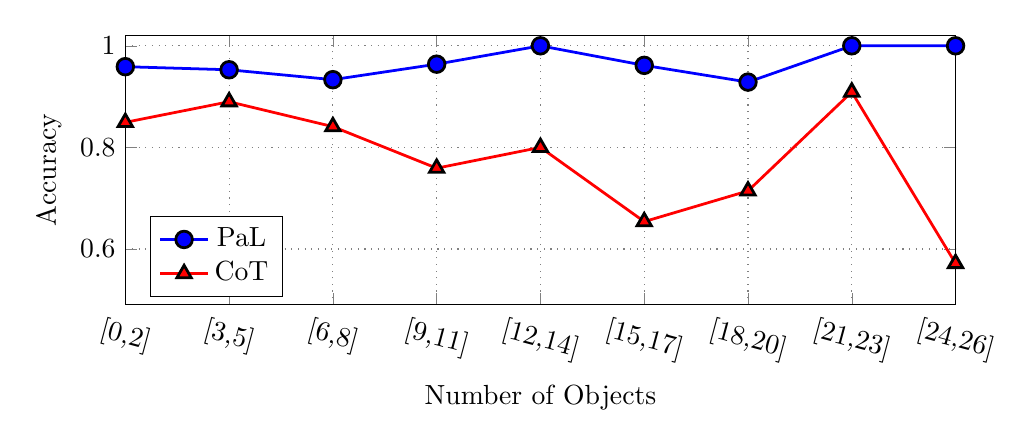
\begin{tikzpicture}
\begin{axis}[xlabel=Number of Objects,    ylabel=Accuracy, xmin=0, xmax=8, xticklabels={[0\text{,}2], [3\text{,}5], [6\text{,}8], [9\text{,}11], [12\text{,}14], [15\text{,}17],[18\text{,}20], [21\text{,}23],  [24\text{,}26]},   ymin=0.49, ymax=1.02,    xtick={0,1,2,3,4,5,6,7,8},    ytick={0.6,0.8,1.0},    legend pos=south west,    
xticklabel style = {rotate=-15},
grid = major, major grid style={dotted,gray},
height=5cm,
width=1\linewidth,
]

\addplot[    color=blue,    mark=*,  line width=1pt , mark size=3pt,
mark options={solid, fill=blue, draw=black}
]
    coordinates {
    (0,0.958904109589041) (1,0.9528145695364238) (2,0.9333333333333333) (3,0.963855421686747) (4,1.0) (5,0.9615384615384616) (6,0.9285714285714286) (7,1.0) (8,1.0)
    };
    \addlegendentry{PaL}
    
\addplot[    color=red,    mark=triangle*,  line width=1pt , mark size=3pt,
    mark options={solid, fill=red, draw=black}
]
    coordinates {
    (0,0.8493150684931506) (1,0.8899006622516556) (2,0.8408602150537634) (3,0.7590361445783133) (4,0.8) (5,0.6538461538461539) (6,0.7142857142857143) (7,0.9090909090909091) (8,0.5714285714285714)
    };
    \addlegendentry{CoT}
\end{axis}
\end{tikzpicture}
\caption{The solve rate on \textsc{Colored Objects} with respect to the number of objects included in the test question. }\label{fig:count_breakdown}
\end{figure} 

\pgfplotstableread[row sep=\\,col sep=&]{
    n & data \\
    code-cushman-001    &  13.6 \\
    code-davinci-001    &   22.3 \\
    code-davinci-002    &  19.8 \\
    }\relativeimprovedata

\pgfplotstableread[row sep=\\,col sep=&]{
    dataset & cot  & pal  \\
    text-davinci-001   &  26.5  & 8.6 \\
    text-davinci-002    &  46.9  & 65.8  \\
    text-davinci-003 &  65.3  & 69.8  \\
}\textpaldata
\begin{figure*}[t]
\begin{minipage}{0.45\textwidth}
  \definecolor{nicecyan}{HTML}{1DA2FF}
  \definecolor{nicegreen}{HTML}{0F9D58}
  \definecolor{nicepurple}{HTML}{AB30C4}

    \begin{tikzpicture}[scale=1]
      \begin{axis}[
        ylabel={Solve rate},
        ylabel style={font=\footnotesize},
        ylabel near ticks,
        legend style={at={(0,1)},anchor=north west,mark size=3pt, inner xsep=1pt, inner sep=0pt},
            legend cell align={left},
        legend cell align={left},
        ymin=0, ymax=80,
        symbolic x coords={code-cushman-001, code-davinci-001, code-davinci-002},
        xtick=data,
        ytick={0,20,40,60,80},
          grid = major,
          major grid style={dotted,gray},
          height=5cm,
          width=1.05\textwidth,
          enlarge x limits=0.1,
          ]
          
          
          \addplot[color=blue, solid, mark options={solid, fill=blue, draw=black}, mark=*, line width=1pt, mark size=3pt, visualization depends on=\thisrow{alignment} \as \alignment, nodes near coords, point meta=explicit symbolic,
          every node near coord/.style={anchor=\alignment, font=\footnotesize}] 
          table [meta index=2]  {
            x   y       label   alignment
            code-cushman-001  21.7  21.7  -90
            code-davinci-001  31.8  31.8  -45
            code-davinci-002  72.0  72.0  -25
            }; \addlegendentry{\ours}
            
            \addplot[color=red, solid, mark options={solid, fill=red, draw=black}, mark=triangle*, line width=1pt, mark size=3pt, visualization depends on=\thisrow{alignment} \as \alignment, nodes near coords, point meta=explicit symbolic,
            every node near coord/.style={anchor=\alignment, font=\footnotesize}] 
            table [meta index=2]  {
            x   y       label   alignment
            code-cushman-001  19.1  19.1  170
            code-davinci-001  26.0  26.0  180
            code-davinci-002  60.1  60.1  90
            };
            \addlegendentry{\cotp}
  
            \addplot[ybar=2pt,color=nicepurple, solid, line width=1pt, visualization depends on=\thisrow{alignment} \as \alignment, nodes near coords, point meta=explicit symbolic,
            every node near coord/.style={anchor=\alignment, font=\footnotesize},
            bar width=24pt,
            fill=nicepurple!20, text=black,
            mark=square*, mark options={solid, fill=nicepurple, draw=black}, mark size=0pt,
            ybar interval legend, 
            forget plot,
            ] 
            table [meta index=2]  {
            x   y       label   alignment
            code-cushman-001  13.6  13.6\%  90
            code-davinci-001  22.3  22.3\%  90
            code-davinci-002  19.8  19.8\%  90
            };

            \addplot[ybar=2pt,color=nicepurple, solid, line width=1pt, visualization depends on=\thisrow{alignment} \as \alignment, nodes near coords, point meta=explicit symbolic,
            every node near coord/.style={anchor=\alignment, font=\footnotesize},
            bar width=2pt,
            fill=nicepurple!20, text=black,
            mark=square*, mark options={solid, fill=nicepurple!20, draw=black}, mark size=0pt,
            draw=none,
            ybar interval legend, 
            ] 
            table [meta index=2]  {
            x   y       label   alignment
            code-davinci-002  -1  {}  90
            };
            \addlegendentry{Relative Improvement}

          \end{axis}
  \end{tikzpicture}
  \caption{\ours with different models on \gsm: though the absolute accuracies with \texttt{code-cushman-001} and \texttt{code-davinci-001} are lower than \texttt{code-davinci-002}, the relative improvement of \ours over \cotp is consistent across models.
  }
  \label{fig:palsmalllms} 
\end{minipage}
\hfill
\begin{minipage}{0.48\textwidth}
  \definecolor{nicecyan}{HTML}{1DA2FF}
  \definecolor{nicegreen}{HTML}{0F9D58}
  \definecolor{niceorange}{HTML}{F8BA02}
  \definecolor{nicered}{HTML}{FF2601}
  \centering
  \begin{tikzpicture}
          \begin{axis} [ybar=2pt,
          bar width=20pt,
              enlarge x limits=0.2,
              legend style={at={(0,1)},anchor=north west,mark size=2pt,
                /tikz/every even column/.append style={column sep=6mm},
                legend columns=-1},
              legend cell align={left},
              symbolic x coords={text-davinci-001,text-davinci-002,text-davinci-003},
              ymin=0, ymax=80,
              ytick={0,20,40,60,80},
              xtick=data,
              grid = major,
              major grid style={dotted,gray},
              height=5cm,
              width=1.05\textwidth,
              yticklabel style={
              /pgf/number format/fixed,
              /pgf/number format/precision=2,
              nodes near coords={\pgfkeys{/pgf/fpu}\pgfmathparse{\pgfplotspointmeta}\pgfmathprintnumber{\pgfmathresult}},
              every node near coord/.append style={font=\footnotesize, color=black},
              nodes near coords align={vertical},
              },
              ] 

              \addplot[black, fill=red,line width=1pt] table[x=dataset,y=cot]{\textpaldata};
              \addplot[black, fill=blue,line width=1pt] table[x=dataset,y=pal]{\textpaldata};
              \legend{\cotp, \ours}
          \end{axis}
  \end{tikzpicture}
      \caption{\ours with NL LMs  on \gsm: though \cotp outperforms \ours with \texttt{text-davinci-001}, once the base LM is sufficiently strong, \ours is beneficial with \texttt{text-davinci-002} and \texttt{text-davinci-003} as well. That is, \ours is not limited to code-LMs only.
      }
    \label{fig:paltextlm} 
\end{minipage}
\end{figure*} \paragraph{Is \ours sensitive to the complexity of the question?}
We examined how the performance of \ours and \cotp change as the complexity of the input question grows, measured as the number of objects in the question of \textsc{Colored Objects}. 
As shown in \Cref{fig:count_breakdown}, \ours is superior \cotp
across all input lengths. As the number of objects in the question increases, 
\cotp's accuracy is unstable and drops, while \ours remains consistently close to 100\%. 
More analysis on the token-level predictions can be found in Appendix \ref{sec:token_analysis}.

\section{Analysis}
\label{sec:analysis}

\begin{figure*}[t]
    \definecolor{nicecyan}{HTML}{1DA2FF}
    \definecolor{nicegreen}{HTML}{0F9D58}
    \definecolor{niceorange}{HTML}{F8BA02}
    \definecolor{nicered}{HTML}{FF2601}
    \centering
    \begin{tikzpicture}
            \begin{axis} [ybar=2pt,
                bar width=22pt,
                enlarge x limits=0.2,
                legend style={at={(0.5,1)},anchor=north,mark size=2pt,
                  /tikz/every even column/.append style={column sep=6mm},
                  font=\small, legend columns=-1},
                legend cell align={left},
                symbolic x coords={Colored Objects,Date,Penguins},
                ymin=60, ymax=103,
                ytick={60,70,80,90,100},
                ylabel style={font=\footnotesize},
                xtick=data,
                grid = major,
                major grid style={dotted,gray},
                height=5cm,
                width=0.95\textwidth,
                yticklabel style={
                /pgf/number format/fixed,
                /pgf/number format/precision=2,
                nodes near coords={\pgfkeys{/pgf/fpu}\pgfmathparse{\pgfplotspointmeta}\pgfmathprintnumber{\pgfmathresult}},
                every node near coord/.append style={font=\footnotesize, color=black},
                nodes near coords align={vertical},
                },
                scaled y ticks=false
                ] 

                \addplot[black, fill=red,line width=1pt] table[x=dataset,y=cot]{\ablationdata};
                \addplot[black, fill=blue,line width=1pt] table[x=dataset,y=pal]{\ablationdata};
                \addplot[black, fill=niceorange,line width=1pt] table[x=dataset,y=palcomment]{\ablationdata};
                \addplot[black,fill=nicegreen,line width=1pt] table[x=dataset,y=palvarcomment]{\ablationdata};
                \legend{\cotp, \ours, , }
            \end{axis}
    \end{tikzpicture}
        \caption{Ablation study of \ours prompt formats. We consider the original \ours prompt, it with natural language comments removed~(), and further variable names replaced with random character~(). As a reference, we also show the \cotp performance~(blue).}
      \label{fig:ablation} 
    \end{figure*} 
\paragraph{Does \ours work with weaker LMs?} In all our experiments in \Cref{sec:results}, \ours used the \texttt{code-davinci-002} model; but can \ours work with weaker models of code? We compared \ours with \cotp when both prompting approaches use the same weaker base LMs \texttt{code-cushman-001} and \texttt{code-davinci-001}. As shown in \Cref{fig:palsmalllms}, even though the absolute accuracies of \texttt{code-cushman-001} and \texttt{code-davinci-001} are lower, the relative improvement of \ours over \cotp remains consistent across models.
This shows that \ours can work with weaker models, while its benefit scales elegantly to stronger models as well.

\paragraph{Does \ours work with LMs of natural language?} We also experimented with \ours using the \texttt{\emph{text}-davinci} series. \Cref{fig:paltextlm} shows the following interesting results: when the base LM's ``code modeling ability'' is weak (using \texttt{text-davinci-001}), \cotp performs better than \ours. However, once the LM's code modeling ability is sufficiently high (using \texttt{text-davinci-002} and \texttt{text-davinci-003}), \ours outperforms \cotp, and \ours performs almost as \ours.
This shows that \ours is not limited to LMs of code, but it can work with LMs that were mainly trained for natural language, if they have a sufficiently high coding ability.


\paragraph{Is \ours better because of the Python prompt or because of the interpreter?} We experimented with generating Python code, while requiring the neural LM to ``execute'' it as well, without using an interpreter, following \citet{scratchpad2021,cocogen}. We created prompts that are similar to \ours's, except that they \emph{do include} the final answer. 
This resulted in a 23.2 solve rate on \gsm, much lower than \ours~(72.0), and only 4.5 points higher than \direct.
These results reinforce our hypothesis that the main benefit of \ours comes from the synergy with the interpreter, and not only from having a better prompt.
Additional details are provided in \Cref{sec:gsmappendixanalysis}.
For additional discussion on the advantages of code-prompts over textual-prompts, see \Cref{sec:token_analysis}.

\paragraph{Do variable names matter?} In all our experiments, we used meaningful variable names in the \ours prompts, to ease the model's grounding of variables to the entities they represent.
For the Python interpreter, however, variable names are meaningless.
To measure the importance of meaningful variable names, we experimented with two prompts variants:
\begin{enumerate}
    \item  -- the \ours prompt without intermediate NL comments.
    \item  -- the \ours prompt without intermediate NL comments \emph{and} with variable names substituted with random characters.
\end{enumerate}


The results are shown in \autoref{fig:ablation}. 
In \textsc{Colored Objected} and \textsc{Date}, 
removing intermediate NL comments but keeping meaningful variable names () -- slightly reduces the results compared to the full \ours prompt, but it still achieves higher accuracy than the baselines \cotp. Removing variable names as well () further decreases  accuracy, and performs worse than \cotp. Since variable names have an important part in code quality \citep{gellenbeck1991investigation, takang1996effects}, meaningful variable names are only expected to ease reasoning for Codex, which was trained on mostly meaningful names, as was also found by \citet{cocogen}.





 
\section{Related Work}
\label{sec:extended_related_work}
\paragraph{Prompting}
Few-shot prompting~\cite{brown2020language} has been shown to be an effective approach for a variety of tasks~\citep{liu2021pre} ranging from text-~\citep{gem,reif2021recipe,flan,bigscience} to code-generation \citep{chen_evaluating_2021}. 
Methods such as chain-of-thought prompting~(\cotp) have further unlocked a variety of reasoning tasks, boosting the performance of models on a variety of benchmarks.
Nevertheless, all previous approaches suffer from inaccuracy in arithmetic calculation and incorrect reasoning \citep{minerva,hendrycks2021measuring,cotanalysis2022}.  \ours avoids these problems by offloading the calculation and some of the reasoning to a Python interpreter, which is correct by construction, given the right program.
Further, not only that \ours can improve the standard chain-of-thought, it can improve least-to-most prompting \citep{zhou2022least} as well, as we show in \Cref{appendix:l2m}.




\paragraph{LMs with external tools}
Several prior works have equipped neural models with specialized modules. For example, \citet{cobbe2021training} employ a calculator for arithmetic operations as a post hoc processing, and \citet{demeter2020just_add_functions} add specialized modules for generating cities and dates.
Unlike these works, \ours generates code for a Python interpreter, which is general enough to handle both arithmetic calculations and dates, without specialized modules and ad-hoc fixes.
\citet{palm:arxiv} and \citet{wei2022chain} have also experimented with external calculators; however, the  calculator had improved Codex by only 2.3\% (absolute) on \gsm and improved \largepalm by 1.7\%, while \ours improves Codex by 6.4\% on the same benchmark (\Cref{sec:math_result}).
Similarly to our work, \citet{palm:arxiv} have also experimented with generating Python code for solving the \gsm benchmark, but their experiments resulted in \emph{lower} accuracy than the standard \largepalm that uses chain-of-thought. 
\citet{pi2022reasoning} pretrain the model on execution results of random expressions on a calculator, 
instead
of using the solver at test time as well. While their model can hypothetically perform arithmetic better than other pretrained LMs, their results on the SVAMP benchmark are much lower: 57.4\% using a T5-11B model, while PAL achieves 79.4\% on the same benchmark without any specialized pretraining.

Shortly after a preprint of our work was submitted to arXiv, another related work on ``program of thought prompting'' \cite{chen2022program} was also submitted to arXiv. Their method is conceptually similar to ours, but PoT (1) only demonstrates efficacy on mathematical problems, whereas we demonstrate gains on symbolic and algorithmic benchmarks as well, and (2) chose benchmark-specific prompt examples, while we used the same prompt examples as previous work, to disentangled the benefit of our approach from the benefit of the choice of examples.




\paragraph{Semantic parsing} 
Our work can also be seen as a very general form of semantic parsing, where instead of parsing into strict domain-specific languages, the model generates free-form Python code.
Some works constrain the decoder using a Context-Free Grammar (CFG) to generate a domain-specific meaning representation \citep{shin2021few} or a canonical utterance, which can be converted to a Lisp-like meaning representation \citep{shin2021constrained}. In contrast, \ours does not require any constraining or domain-specific representations other than Python code. Further, LMs that were pretrained on Python are abundant compared to other domain-specific languages, making Python code a much more preferable representation.
\citet{andor2019giving} generate task-specific arithmetic operations for reading comprehension tasks; 
\citet{gupta2019neural} design neural modules such as \texttt{count} to deal with arithmetic operations. 
\ours generalizes these works by generating general Python programs, without the need for defining specialized modules.
The closest work to ours technically may be Binder \citep{cheng2022binding}, but it addressed mostly answering questions about tables using SQL and SQL-like Python.



 \section{Conclusion}
\label{sec:conclusion}


We introduce \ours, a new method for natural language reasoning, using \emph{programs} as intermediate reasoning steps. 
Differently from existing LM-based reasoning approaches, the main idea is to offload solving and calculating to an external Python interpreter, instead of using the LLM for both understanding the problem \emph{and} solving. This results in a final answer that is guaranteed to be accurate, given the correctly predicted programmatic steps.
We demonstrate this seamless synergy between an LLM and a Python interpreter across 13 tasks from BIG-Bench Hard and other benchmarks. In all these benchmarks, \ours outperforms larger LLMs such as \largepalm which use the popular ``chain-of-thought'' method
and sets new state-of-the-art accuracy on all of them. 
We believe that these results unlock exciting directions for future neuro-symbolic AI reasoners.




 \let\oldaddcontentsline\addcontentsline
\renewcommand{\addcontentsline}[3]{}
\bibliography{main}
\let\addcontentsline\oldaddcontentsline
\bibliographystyle{icml2022}
\newpage
\appendix
\onecolumn

\doparttoc
\faketableofcontents

\addcontentsline{toc}{section}{Appendix}
\part{Appendix}
\parttoc

\clearpage

\section{Alternative Prompts without Meaningful Variable Names}
\label{sec:gsm:additional_analysis}
\begin{figure*}[!ht]
\centering
\begin{subfigure}[t]{.95\textwidth}
\centering
 \begin{minted}[fontsize=\footnotesize,framesep=1pt,frame=single,autogobble,breaklines,breaksymbolleft=\;,escapeinside=||]{python}
|\varref{a}| = 23
|\varref{b}| = 5
|\varref{c}| = 3
|\varref{d}| = |\varref{b}| * |\varref{c}|
|\varref{e}| = |\varref{a}| - |\varref{d}|
print(e)
\end{minted}
\label{fig:gsmablations:badnames}
\caption{Structured explanation with uninformative variable names~(\ours\ - \texttt{var})}

\end{subfigure}\hfill\\
\begin{subfigure}[t]{.95\textwidth}
\centering
 \begin{minted}[fontsize=\footnotesize,framesep=1pt,frame=single,autogobble,breaklines,breaksymbolleft=\;,escapeinside=||]{python}
# Olivia has 23. She bought five bagels for \4^{th}5^{th}23. She bought five bagels for \\sim100.00 and currently 10\% off.  If he buys 2 boxes of contact, how much will each pair of contacts cost? &
  90 contacts come in 1 box. Each box is \100.00. If he buys 2 boxes, then he will have 2 x 90 = 180 contacts. 180 contacts cost 2 x \200.00. So each pair of contacts costs \1.11. The answer is \5451440 and currently 10\% off. So each box is \4906296. If he buys 2 boxes of contact, he will have 2 * 90 = 180 contacts. So each pair of contacts will cost \2725849. The answer is \1.50. How much did the chef spend? &
  The chef bought 4 bags of onions. Each bag weighs 50 pounds. So the total weight is 4 * 50 = 200 pounds. A pound of onions cost \409201. So 200 pounds of onions cost 200 * 409201 = \81840200. &
  Yes \\
A bag has a 5\% discount. If it is marked \3921772.0722 is \3730654.0682 &
  Yes \\
A basket of green food costs \18. If you buy 3 baskets of green food and red food, how much will you have to pay in total if you get \2 off for each basket of red food. So you get 3 * 2 = 6 dollars off. So you pay 75 + 54 - 6 = 123 dollars. The answer is 123. &
  A basket of green food costs 9412763 dollars. A basket of red food costs 18 dollars. If you buy 3 baskets of green food and red food, you will have to pay 9412763 * 3 + 18 * 3 = 28238280 dollars. If you get 2 dollars off for each basket of red food, you will have to pay 28238280 - 18 * 2 = 28238244 dollars. The answer is 28238244 &
  No \\
A bumper car rink has 12 red cars. They have 2 fewer green cars than they have red cars. They have 3 times the number of blue cars as they have green cars. The rink also has yellow cars.  If the rink has 75 cars in total how many yellow cars do they have? &
  There are 12 red cars. There are 2 fewer green cars than red cars. So there are 12 - 2 = 10 green cars. There are 3 times as many blue cars as green cars. So there are 3 * 10 = 30 blue cars. There are 12 + 10 + 30 = 52 cars that are not yellow. So there are 75 - 52 = 23 yellow cars. The answer is 23. &
  The rink has 9318738 red cars. They have 2 fewer green cars than red cars. So they have 9318738 - 2 = 9318736 green cars. They have 3 times the number of blue cars as green cars. So they have 3 * 9318736 = 27956208 blue cars. The total number of cars is 75. So the number of yellow cars is 75 - 9318738 - 9318736 - 27956208 = -55,828,829. The answer is -55,828,829 &
  Yes \\
  \bottomrule
\end{tabular}
\caption{Analysis of generations from \codex. Manual analysis of 25 randomly generated thoughts reveals that 16 out of 25 thoughts were identical, whereas others were close paraphrases.}
\label{tab:gsmhard:cotanalysis}
\end{table}



\newpage
\clearpage

\subsection{Creating \gsmhard}\label{appendix:create_gsmhard}
While replacing numbers in the question is easy using pattern matching, a more challenging aspect is recalculating the correct answer.
\gsm evaluation set contains 1319 samples, which is prohibitively expensive to perform manual re-calculation. 
Instead, we leverage \ours to assist obtaining the correct answers.
For 71\% of the examples where \ours is correct on \gsm, we utilize the generated program and replace the initial value with the larger values.
For example, if we create a harder version of the problem in~\autoref{fig:mathsprompt} by replacing \15687 dollars, we correspondingly replace \inlineCode{money\_initial=23} to \inlineCode{money\_initial=15678}.
Running the program could automatically produce the correct answer of the harder question.
Notably, this annotation process assumes that a program that produces a correct answer to a \gsm question indicates the correctness of the program itself. 
While this is not guaranteed due to possible spurious correlations, we manually checked 25 programs and found all of them are correct. 
For the incorrect 29\% of the cases, we run \ours again and perform nucleus sampling~\citep{holtzman2019curious} with temperature 0.7, and repeat the above process if any correct solution is found.
Finally, the authors manually annotate the correct answer for  remaining cases that \ours was not able to solve after 100 iterations.


\subsection{\gsmhard Analysis}
\label{sec:gsmhardanalysis}

\Cref{tab:gsmhard:cotanalysis} shows thoughts generated with \cotp on \gsm and \gsmhard.
A manual analysis reveals that a majority of the generated thoughts (16/25) were identical for \gsm and \gsmhard, indicating that larger numbers primarily diminish performance due to failure of \llm to do arithmetic..

\newpage
\section{Generalization of PAL to Least-to-Most Prompting}
\label{appendix:l2m}
\begin{figure*}[!h]
\centering

\begin{subfigure}[t]{.95\textwidth}
\centering
\begin{minted}[fontsize=\footnotesize,breaklines,framesep=1pt,frame=single]{text}
Q: Four years ago, Kody was only half as old as Mohamed. If Mohamed is currently twice 30 years old, how old is Kody?
A: To answer the question "How old is Kody?", we need to know: "How old is Mohamed?", "How old was Mohamed four years ago?", "How old was Kody four years ago?".
\end{minted}
\caption{Least-to-Most Math Reducing Prompt}
\end{subfigure}

\begin{subfigure}[t]{.95\textwidth}
\centering
\begin{minted}[fontsize=\footnotesize,breaklines,framesep=1pt,frame=single]{text}
Four years ago, Kody was only half as old as Mohamed. If Mohamed is currently twice 30 years old, how old is Kody?

Q: How old was Mohamed four years ago?
A: We were told that Mohamed is currently twice 30 years old, so he is currently 30 * 2 = 60 years old. That means that four years ago he must have been 60 - 4 = 56 years old. The answer is 56.

Q: How old is Kody?
A: Four years ago, Kody was half as old as Mohamed, so Kody must have been 56 / 2 = 28 years old then. Since Kody was 28 years old four years ago, she must now be 28 + 4 = 32 years old. The answer is 32.
\end{minted}
\caption{Least-to-Most Math Solving Prompt}
\end{subfigure}

\begin{subfigure}[t]{.95\textwidth}

 \begin{minted}[fontsize=\footnotesize,framesep=1pt,frame=single,autogobble,breaklines,breaksymbolleft=\;,escapeinside=||]{python}
# Four years ago, Kody was only half as old as Mohamed. If Mohamed is currently twice 30 years old, how old is Kody?

# How old was Mohamed four years ago?
mohamed_age_current = 30 * 2
mohamed_age_4_years_ago = mohamed_age_current - 4

# Final Question: How old is Kody?
kody_age_4_years_ago = mohamed_age_4_years_ago / 2
kody_age_current = kody_age_4_years_ago + 4
answer = kody_age_current
\end{minted}
\caption{\ours Math Solving Prompt}
\end{subfigure}
\caption{Prompts for Math data sets.}
\label{fig:quco-l2m-solve-prompt}
 \end{figure*}

Previous experiments focus on the \cotp technique. This section examines if \ours generalizes to other prompt types. We consider a strong alternative prompting strategy \tomost 
\cite{zhou2022least}. \tomost solves problems in two stages, problem-reducing and problem-solving. Problem reducing stage turns the problem into sub-problems, and the solving stage solves them sequentially. It keeps two prompts, each for an individual stage. To patch \tomost prompts with \
\ours, we adopt a simple and straightforward approach: we note that problem reduction requires logically thinking in NL while solving requires the precision that PL offers. We therefore keep the original reducing prompts while only turning solution segments in the solving scripts in PL. We show an example reducing prompt, original solving prompt, and \ours solving prompt in \autoref{fig:quco-l2m-solve-prompt}. Note that one unique property of \ours solving can naturally use previous questions' answers as the symbol values are shared. In comparison, the original solving script needs to explicitly re-cite answers from previous answers.

\begin{table}[h!]
\centering
\begin{tabular}{@{}lcc@{}}
\toprule
Dataset (500 examples)                 & \tomost & \tomost + \ours \\ \midrule
\gsm               & 67.2  & \textbf{72.8}                     \\
\svamp                 & 75.2     & \textbf{78.2}                     \\ \bottomrule
\end{tabular}
\caption{Results on \gsm and \svamp with \tomost and \tomost with \ours solving prompt.}
\label{tab:quco-l2m:results}
\end{table}

For our analysis, we consider the Math data sets \gsm, and \svamp as \citet{zhou2022least} found Least-to-Most helps solve complex math problems. We patch the \gsm prompt from the \citet{zhou2022least} into \ours. Note that the other tasks in \citet{zhou2022least}, like ``concatenating last letters" from several words, require simple routines and are trivially solvable by \ours. We experiment with subsets of 500 examples and record results in \autoref{tab:quco-l2m:results}. Here we see \ours can take advantage of the problem decomposition offered by the \tomost reducing and further leverage the arithmetic capability in the Python runtime to achieve additional performance gains.

\clearpage

\section{Prompts}
\label{sec:appendixprompts}
We show here example \ours prompts we used for each data set. We show one example for each of the few-shot prompts. The fulls prompt can be found in our released code.

\subsection{Reasoning about Colored Objects}
\begin{figure*}[!h]
\centering
\begin{subfigure}[t]{.95\textwidth}

 \begin{minted}[fontsize=\footnotesize,framesep=1pt,frame=single,autogobble,breaklines,breaksymbolleft=\;,escapeinside=||]{python}
# Q: On the table, you see a bunch of objects arranged in a row: a purple paperclip, a pink stress ball, a brown keychain, a green scrunchiephone charger, a mauve fidget spinner, and a burgundy pen. What is the color of the object directly to the right of the stress ball?
# Put objects into a list to record ordering
objects = []
objects += [('paperclip', 'purple')] * 1
objects += [('stress ball', 'pink')] * 1
objects += [('keychain', 'brown')] * 1
objects += [('scrunchiephone charger', 'green')] * 1
objects += [('fidget spinner', 'mauve')] * 1
objects += [('pen', 'burgundy')] * 1
# Find the index of the stress ball
stress_ball_idx = None
for i, object in enumerate(objects):
    if object[0] == 'stress ball':
        stress_ball_idx = i
        break
# Find the directly right object
direct_right = objects[stress_ball_idx+1]
# Check the directly right object's color
direct_right_color = direct_right[1]
answer = direct_right_color
\end{minted}
\end{subfigure}
\end{figure*}



\newpage
\subsection{Penguins in a Table}
\label{app:sec:penguins}
\begin{figure*}[!h]
\centering
\begin{subfigure}[t]{.95\textwidth}
\begin{minted}[fontsize=\footnotesize,framesep=1pt,frame=single,autogobble,breaklines,breaksymbolleft=\;,escapeinside=||]{python}
"""Q: Here is a table where the first line is a header and each subsequent line is a penguin: name, age, height (cm), weight (kg)  Louis, 7, 50, 11 Bernard, 5, 80, 13 Vincent, 9, 60, 11 Gwen, 8, 70, 15 For example: the age of Louis is 7, the weight of Gwen is 15 kg, the height of Bernard is 80 cm.  We now add a penguin to the table: James, 12, 90, 12
How many penguins are less than 8 years old?
"""
# Put the penguins into a list.
penguins = []
penguins.append(('Louis', 7, 50, 11))
penguins.append(('Bernard', 5, 80, 13))
penguins.append(('Vincent', 9, 60, 11))
penguins.append(('Gwen', 8, 70, 15))
# Add penguin James.
penguins.append(('James', 12, 90, 12))
# Find penguins under 8 years old.
penguins_under_8_years_old = [penguin for penguin in penguins if penguin[1] < 8]
# Count number of perguins under 8.
num_penguin_under_8 = len(penguins_under_8_years_old)
answer = num_penguin_under_8
\end{minted}
\end{subfigure}
\caption{}
\label{fig:penguins}
\end{figure*}
 
 
 \newpage
\subsection{Date Understanding}
\begin{figure*}[!ht]
\centering
\begin{subfigure}[t]{.95\textwidth}

 \begin{minted}[fontsize=\footnotesize,framesep=1pt,frame=single,autogobble,breaklines,breaksymbolleft=\;,escapeinside=||]{python}
# Q: 2015 is coming in 36 hours. What is the date one week from today in MM/DD/YYYY?
# If 2015 is coming in 36 hours, then today is 36 hours before.
today = datetime(2015, 1, 1) - relativedelta(hours=36)
# One week from today,
one_week_from_today = today + relativedelta(weeks=1)
# The answer formatted with one_week_from_today.strftime('\end{minted}
\label{fig:date:prompt}
\end{subfigure}
\end{figure*}



\newpage
\subsection{Math}
\begin{figure*}[!h]
\centering
\begin{subfigure}[t]{.99\textwidth}
\begin{minted}[fontsize=\footnotesize,framesep=1pt,frame=single,autogobble,breaklines,breaksymbolleft=\;,escapeinside=||]{python}
#Q: Olivia has \3 each. How much money does she have left?
money_initial = 23
bagels = 5
bagel_cost = 3
money_spent = bagels * bagel_cost
money_left = money_initial - money_spent
print(money_left)

#Q: Michael had 58 golf balls. On tuesday, he lost 23 golf balls. On wednesday, he lost 2 more. How many golf balls did he have at the end of wednesday?
golf_balls_initial = 58
golf_balls_lost_tuesday = 23
golf_balls_lost_wednesday = 2
golf_balls_left = golf_balls_initial - golf_balls_lost_tuesday - golf_balls_lost_wednesday
print(golf_balls_left)

#Q: There were nine computers in the server room. Five more computers were installed each day, from monday to thursday. How many computers are now in the server room?

computers_initial = 9
computers_per_day = 5
num_days = 4  # 4 days between monday and thursday
computers_added = computers_per_day * num_days
computers_total = computers_initial + computers_added
print(computers_total)


#Q: If there are 3 cars in the parking lot and 2 more cars arrive, how many cars are in the parking lot?
cars_initial = 3
cars_arrived = 2
total_cars = cars_initial + cars_arrived
print(total_cars)

#Q: Leah had 32 chocolates and her sister had 42. If they ate 35, how many pieces do they have left in total?

leah_chocolates = 32
sister_chocolates = 42
total_chocolates = leah_chocolates + sister_chocolates
chocolates_eaten = 35
chocolates_left = total_chocolates - chocolates_eaten
print(chocolates_left)




\end{minted}
\label{fig:mathsprompt:ourspartone}
\end{subfigure}
\caption{Prompt used for mathematical reasoning (1/2)}
 \end{figure*}

\begin{figure*}[!h]
\centering
\begin{subfigure}[t]{.99\textwidth}
\begin{minted}[fontsize=\footnotesize,framesep=1pt,frame=single,autogobble,breaklines,breaksymbolleft=\;,escapeinside=||]{python}


#Q: Jason had 20 lollipops. He gave Denny some lollipops. Now Jason has 12 lollipops. How many lollipops did Jason give to Denny?
jason_lollipops_initial = 20
jason_lollipops_after = 12
denny_lollipops = jason_lollipops_initial - jason_lollipops_after
print(denny_lollipops)



#Q: There are 15 trees in the grove. Grove workers will plant trees in the grove today. After they are done, there will be 21 trees. How many trees did the grove workers plant today?
trees_initial = 15
trees_after = 21
trees_added = trees_after - trees_initial
print(trees_added)


#Q: Shawn has five toys. For Christmas, he got two toys each from his mom and dad. How many toys does he have now?

toys_initial = 5
mom_toys = 2
dad_toys = 2
total_received = mom_toys + dad_toys
total_toys = toys_initial + total_received
print(total_toys)

\end{minted}
\label{fig:mathsprompt:oursparttwo}
\end{subfigure}
\caption{Prompt used for mathematical reasoning (2/2)}
 \end{figure*}

\newpage
\clearpage

\subsection{Object Counting}
\begin{figure*}[!h]
\centering
\begin{subfigure}[t]{.95\textwidth}

 \begin{minted}[fontsize=\footnotesize,framesep=1pt,frame=single,autogobble,breaklines,breaksymbolleft=\;,escapeinside=||]{python}
# Q: I have a chair, two potatoes, a cauliflower, a lettuce head, two tables, a cabbage, two onions, and three fridges. How many vegetables do I have?

# note: I'm not counting the chair, tables, or fridges
vegetables_to_count = {
    'potato': 2,
    'cauliflower': 1,
    'lettuce head': 1,
    'cabbage': 1,
    'onion': 2
}
print(sum(vegetables_to_count.values()))


# Q: I have a drum, a flute, a clarinet, a violin, four accordions, a piano, a trombone, and a trumpet. How many musical instruments do I have?

musical_instruments_to_count = {
    'drum': 1,
    'flute': 1,
    'clarinet': 1,
    'violin': 1,
    'accordion': 4,
    'piano': 1,
    'trombone': 1,
    'trumpet': 1
}
print(sum(musical_instruments_to_count.values()))




# Q: I have a chair, two ovens, and three tables. How many objects do I have?

objects_to_count = {
    'chair': 1,
    'oven': 2,
    'table': 3
}
print(sum(objects_to_count.values()))

\end{minted}
\label{appendix:fig:objectcounting:ours}
\end{subfigure}
\caption{Prompt used for \objectcounting.}
\end{figure*}




\newpage
\subsection{Repeat Copy}
\begin{figure*}[!h]
\centering
\begin{subfigure}[t]{.95\textwidth}
 \begin{minted}[fontsize=\footnotesize,framesep=1pt,frame=single,autogobble,breaklines,breaksymbolleft=\;,escapeinside=||]{python}
# Q: Repeat the word duck four times, but halfway through also say quack

result = []
for i in range(1, 5):
    result.append("duck")
    if i == 2:
        result.append("quack")
print(" ".join(result))


# Q: Print boolean eleven times, but after the 3rd and 8th also say correct

result = []
for i in range(1, 12):
    result.append("boolean")
    if i == 3 or i == 8:
        result.append("correct")
print(" ".join(result))

# Q: say java twice and data once, and then repeat all of this three times.

result = []
tmp = ["java", "java", "data"]
for i in range(3):
    result.extend(tmp)
print(" ".join(result))


# Q: ask a group of insects in what family? four times. after the fourth time say The happy family

result = []
tmp = []
for i in range(1, 5):
    tmp.append("a group of insects in what family?")
tmp.append("The happy family")
result.extend(tmp)
print(" ".join(result))

\end{minted}
\label{fig:repeatcopy:ours}
\end{subfigure}
\caption{Prompt used for \repeatcopy.}
 \end{figure*}


  
  
  

\clearpage
\section{Success and Failure Modes in Symbolic Tasks}
\subsection{Colored Objects}
\begin{figure*}[!h]
    \centering
    
    \begin{subfigure}[t]{.95\textwidth}
    
     \begin{minted}[fontsize=\footnotesize,framesep=1pt,frame=single,autogobble,breaklines,breaksymbolleft=\;,escapeinside=||]{python}
    # Find non-gold items to the right of the pencil
    non_gold = [object for object in objects[i+1:] if object[1] != 'gold']
    \end{minted}
    \caption{Snippet of \ours doing a filter operation.}
    \label{fig:color-example:1}
    \end{subfigure}
    
    \begin{subfigure}[t]{.95\textwidth}
     \begin{minted}[fontsize=\footnotesize,framesep=1pt,frame=single,autogobble,breaklines,breaksymbolleft=\;,escapeinside=||]{python}
    # Remove all pink objects
    non_pink = [object for object in objects if object[1] != 'pink']
    
    # Count number of crayons
    crayons = [object for object in non_pink if object[0] == 'crayon']
    answer = len(crayons)
    \end{minted}
    \caption{Snippet of \ours composing multiple operations.}
    \label{fig:color-example:2}
    \end{subfigure}
    
    \caption{Example model generation snippets on Reasoning about Color Object.}
    \label{fig:color-example}
     \end{figure*}

     By manually examining the the model outputs, we observe that \ours often performs better on questions that involve \emph{counting} objects that satisfy one or several conditions. 
     For example,  \cotp fails in the following example: \textit{``On the desk, you see a bunch of items arranged in a row: a gold textbook, a purple puzzle, a teal necklace, and a silver pencil. How many non-gold items do you see to the right of the pencil?''}.
     With pure NL reasoning, a \llm can easily lose track of the objects and output the wrong answer of \textit{``The number of non-gold items to the right of the pencil is two. So the answer is two.''} 

     In comparison, \ours is able to accurately construct the object lists with correct order and attributes. 
     Further, it can precisely leverage the simple yet complete PL syntax: it composes routines with functional operators from elementary builtin operation/operators. 
     \autoref{fig:color-obj:prompt} lists the last a few lines of the solution to the question described above generated by \ours, which perform filtering over objects. 
     \ours can further compose such operations across multiple reasoning steps as shown in \autoref{fig:color-example:2}, where it first filters out all pink objects and then scans the remaining to count crayons.
     Other reasoning such as ``how many objects are left after filtering'' can be easily tackled precisely with an runtime. 

\subsection{Penguins in a Table} 
 \begin{figure*}[!h]
\centering

\begin{subfigure}[t]{.95\textwidth}
\centering
\begin{minted}[fontsize=\footnotesize,breaklines,framesep=1pt,frame=single]{text}
...This question focuses on age. We know the following: Louis is 7 years old, Bernard is 5 years old, Vincent is 9 years old, and Gwen is 8 years old.Now, we add James to this table: James is 12 years old. We then delete the penguin named Bernard from the table.The penguins that are less than 8 years old are Louis and Bernard. There are 2 penguins less than 8 years old. So the answer is 2.
\end{minted}
\end{subfigure}

\begin{subfigure}[t]{.95\textwidth}

\begin{minted}[fontsize=\footnotesize,framesep=1pt,frame=single,autogobble,breaklines,breaksymbolleft=\;,escapeinside=||]{python}
...
# Delete penguin Bernard.
penguins = [penguin for penguin in penguins if penguin[0] != 'Bernard']
# Find penguins under 8 years old.
penguins_under_8_years_old = [penguin for penguin in penguins if penguin[1] < 8]
# Count number of perguins under 8.
num_penguin_under_8 = len(penguins_under_8_years_old)
answer = num_penguin_under_8
\end{minted}
\end{subfigure}
\caption{Generated Snippets for one question~(\textit{...We then delete the penguin named Bernard from the table. How many penguins are less than 8 years old?}) in Penguins in a Table}.
\label{fig:penguin:snippet}
 \end{figure*}
In this task, we found a typical failure mode of the language is its inability to stably tracks states in its past generation. 
~\autoref{fig:penguin:snippet} lists the generations of \cotp and \ours to the question that contains the removal of a penguin~(\textit{``...We then delete the penguin named Bernard from the table. How many penguins are less than 8 years old?''}).
Although \cotp picks up the critical information that ``penguins that are less then 8 years old are Louis and Bernard'', and that ``Bernard is deleted''. It still fails to aggregate the information properly and infer that there is one penguin less then 8 left in the end. 
In comparison, \ours expresses this dynamic through manipulating a \inlineCode{penguins} list by filtering out the penguin whose name is ``Bernard'', and maintaining  a \inlineCode{penguins\_under\_8\_years\_old} list. It offloads tracking exact the values~(in this case, the length of the list) to the deterministic Python runtime.

\subsection{Date Understanding}
\label{app:sec:date}
\begin{figure*}[h!]
\centering
\begin{subfigure}[t]{.95\textwidth}
\centering
\begin{minted}[fontsize=\footnotesize,breaklines,framesep=1pt,frame=single]{text}
Q: Jane was born on the last day of Feburary in 2001. Today is her 16-year-old birthday. What is the date 24 hours later in MM/DD/YYYY?

A: The last day of February is the 28th, so Jane was born on 02/28/2001. Today is her 16-year old birthday, so today is 02/28/2017. So 24 hours later is 02/29/2017. So the answer is 02/29/2017.
\end{minted}
\label{fig:mainfig:list}
\end{subfigure}

\begin{subfigure}[t]{.95\textwidth}

 \begin{minted}[fontsize=\footnotesize,framesep=1pt,frame=single,autogobble,breaklines,breaksymbolleft=\;,escapeinside=||]{python}
# Q: Jane was born on the last day of Feburary in 2001. Today is her 16-year-old birthday. What is the date 24 hours later in MM/DD/YYYY?
# If Jane was born on the last day of Feburary in 2001 and today is her 16-year-old birthday, then today is 16 years later.
today = datetime(2001, 2, 28) + relativedelta(years=16)
# 24 hours later,
later = today + relativedelta(hours=24)
# The answer formatted with later.strftime('\end{minted}
\end{subfigure}
\caption{Example model generation on Date Understanding.}
\label{fig:date:eggeneration}
 \end{figure*}

We found this especially common when the time deltas are across the month boundary.
We show an example in \autoref{fig:date:eggeneration}. Here with \cotp prompting, the \llm expresses the knowledge of the 28-day-long February, yet it still outputs \textit{02/29/2017} as the final answer. 
With \ours, the actual calendar is accurate as a program handles the operation.
  \end{document}
